\documentclass[preprint,12pt]{elsarticle}


%% The `ecrc' package must be called to make the CRC functionality available
%\usepackage{ecrc}

%% set the volume if you know. Otherwise `00'
%\volume{00}

%% set the starting page if not 1
%\firstpage{1}

%% Give the name of the journal
%\journalname{Expert Systems With Applications}

%% Give the author list to appear in the running head
%% Example \runauth{C.V. Radhakrishnan et al.}
%\runauth{}

%% The choice of journal logo is determined by the \jid and \jnltitlelogo commands.
%% A user-supplied logo with the name <\jid>logo.pdf will be inserted if present.
%% e.g. if \jid{yspmi} the system will look for a file yspmilogo.pdf
%% Otherwise the content of \jnltitlelogo will be set between horizontal lines as a default logo

%% Give the abbreviation of the Journal.  Contact the journal editorial office if in any doubt
%\jid{eswa}

%% Give a short journal name for the dummy logo (if needed)
%\jnltitlelogo{ESWA Logo}

%% Provide the copyright line to appear in the abstract
%% Usage:
%   \CopyrightLine[<text-before-year>]{<year>}{<restt-of-the-copyright-text>}
%   \CopyrightLine[Crown copyright]{2011}{Published by Elsevier Ltd.}
%   \CopyrightLine{2011}{Elsevier Ltd. All rights reserved}
%\CopyrightLine{2013}{Published by Elsevier Ltd.}



%\usepackage{llncsdoc}
\usepackage[figuresright]{rotating}
%\usepackage{makeidx}  % allows for indexgeneration
\usepackage{graphicx}
\usepackage[T1]{fontenc}
\usepackage[english]{babel}
\usepackage[utf8]{inputenc}
% \usepackage{multirow}

\usepackage{natbib}
\usepackage{url}
\usepackage{rotating}

%%%Math
\usepackage{latexsym}
 \usepackage{amsmath}
% \usepackage{amssymb}
% \usepackage{amsthm}
%\usepackage{eurosans}

\usepackage{eurosym}

\usepackage{longtable}

\usepackage{listings}

\usepackage{color}
\usepackage{textcomp}


\definecolor{gray}{gray}{0.5}
\definecolor{green}{rgb}{0,0.5,0}

\usepackage{rotating}
% 
% \usepackage{inconsolata}



\begin{document}


\begin{frontmatter}

%% Title, authors and addresses

%% use the tnoteref command within \title for footnotes;
%% use the tnotetext command for the associated footnote;
%% use the fnref command within \author or \address for footnotes;
%% use the fntext command for the associated footnote;
%% use the corref command within \author for corresponding author footnotes;
%% use the cortext command for the associated footnote;
%% use the ead command for the email address,
%% and the form \ead[url] for the home page:
%%
%% \title{Title\tnoteref{label1}}
%% \tnotetext[label1]{}
%% \author{Name\corref{cor1}\fnref{label2}}
%% \ead{email address}
%% \ead[url]{home page}
%% \fntext[label2]{}
%% \cortext[cor1]{}
%% \address{Address\fnref{label3}}
%% \fntext[label3]{}

%\dochead{}
%% Use \dochead if there is an article header, e.g. \dochead{Short communication}
%% \dochead can also be used to include a conference title, if directed by the editors
%% e.g. \dochead{17th International Conference on Dynamical Processes in Excited States of Solids}


\title{Semantic-based QoS management in Cloud Systems: Current Status and Future Challenges}


 \author[seerc]{Dimitrios Kourtesis}
 \ead{dkourtesis@seerc.org}
 
 \author[seerc]{Jose Mar\'{i}a Alvarez-Rodr\'{i}guez\corref{cor1}}
 \ead{jmalvarez@seerc.org}
 
 \author[seerc]{Iraklis Paraskakis}
 \ead{iparaskakis@seerc.org}
 
 \cortext[cor1]{Corresponding author}
 \address[seerc]{South East European Research Centre (SEERC), 24 Proxenou Koromila Street, Thessaloniki, 54622, Greece}

    
%% use optional labels to link authors explicitly to addresses:

% \author[label3]{Dimitrios Kourtesis}
% \address[label2]{The South East European Research Center, 54622, Thessaloniki, Greece.}
% \ead{dkourtesis@seerc.org}
% 
% \author[label1]{Jose María Alvarez-Rodríguez\corref{cor1}}
% \address[label1]{The South East European Research Center, 54622, Thessaloniki, Greece.}
% \ead{jmalvarez@seerc.org}
% \ead[url]{http://www.seerc.org}
% 
% \author[label2]{Iraklis Paraskakis}
% \address[label2]{The South East European Research Center, 54622, Thessaloniki, Greece.}
% \ead{iparaskakis@seerc.org}






\author{}

\address{}

\begin{abstract}
The concept of Cloud Computing and Service Oriented Architectures have seen a 
dramatic increase of the amount of applications, services, management platforms, 
data, etc. gaining momentum in Information and Communication Technology and more 
specifically in the deployment of the Future Internet. However this explosion 
implies the necessity of new complex methods and techniques to deal with the 
vast heterogeneity of data sources, services or platforms. In this sense Quality 
of Service (QoS) seeks for providing an intelligent environment of 
self-management components based on domain knowledge in which both functional 
and nonfunctional properties of cloud components can be optimized in terms of 
cost, efficiency or reliability easing the transition to an advanced resource 
provisioning process. On the other hand, semantics and ontologies have emerged 
to afford a common and standard data model that eases the interoperability, integration and monitoring of 
knowledge-based systems. Furthermore the Linked Data initiative as practical 
view of the Semantic Web has posed the baseline technology to easily integrate, 
enrich and consume data in a distributed system. Taking into account the 
necessity of an intelligent system to manage QoS in Cloud Systems and the 
emerging application of semantics in different domains, this paper reviews the 
main approaches for semantic-based QoS management as well as the principal methods, techniques and standards for 
processing and exploiting diverse data providing advanced real-time monitoring services. 
A semantic-based framework is also outlined taking into account the QoS requirements and capabilities of semantic technologies and distributed 
datastream processing techniques. Finally a discussion of existing efforts 
and challenges are also provided to suggest future directions.
\end{abstract}

\begin{keyword}
%% keywords here, in the form: keyword \sep keyword
cloud systems \sep quality of service \sep  service oriented architectures \sep  semantics \sep  ontologies \sep  linked data \sep  sensor data \sep  big data 
%% PACS codes here, in the form: \PACS code \sep code

%% MSC codes here, in the form: \MSC code \sep code
%% or \MSC[2008] code \sep code (2000 is the default)

\end{keyword}


\end{frontmatter}

\section{Introduction}
Cloud Computing~\cite{mell2011nist} systems and Service Oriented Architectures (SOA) have 
reached a level of complexity~\cite{Huebscher:2008:SAC:1380584.1380585,Conejero:2012:MSQ:2357487.2357591} that implies the necessity of new methods 
and algorithms to automatically deal with the vast amount of data, variables, 
parameters, etc. that appear in this new realm for the advanced management of 
applications, services or resources. 

In this new environment QoS is playing a relatively minor role but its 
importance, in a wide range of applications scenarios, is likely become more 
crucial than ever before. In recent years and due to the deployment of web 
services a considerable research effort in QoS has been made. However existing 
QoS mechanisms are actually available in a few large scale commercial 
environments and with a limited extent. The main problem lies in the complexity 
of designing QoS models that enables an adequate management of a distributed 
architecture making decisions about resource provisioning, getting feedback for 
the final users, etc. with the objective of avoiding existing ``brute-force''
solutions and overprovisioning. 

Although QoS management has been also widely investigated~\cite{Conejero:2012:MSQ:2357487.2357591} 
in the well-known grid-computing area the emergence of the Cloud Computing paradigm 
brings a new set of open issues: accomplish the  Service Level Agreements (SLAs), predict 
future workload, process large and diverse data streams/logs, make real-time 
decisions, reasoning and inference, dynamic adaptation and provision of 
resources, etc. In the widely-accepted definition~\cite{mell2011nist} of 
he National Institute of Standards and Technology (NIST) QoS 
would be aligned to the concept of ``Measured Service'', see Figure~\ref{fig:qos-intro}, and 
more specifically to define both characteristics applicable to a service and operations 
to deliver some kind of alert or predictive analytics service. 
The aforementioned points are very challenging and should be 
addressed in order to ease an intelligent, flexible and self-managing system of 
cloud-based applications and platforms.


 \begin{figure}[!ht]
\centering
	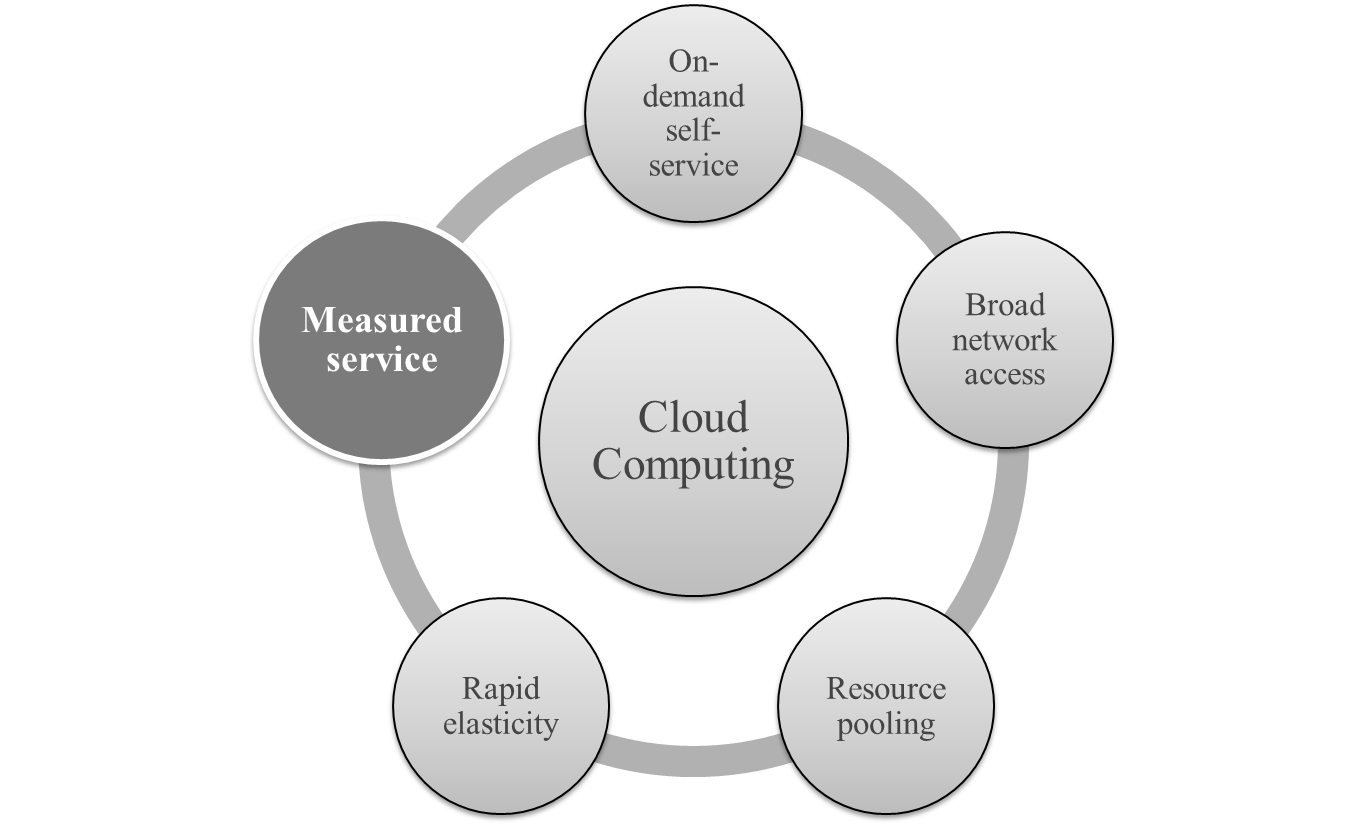
\includegraphics[width=12cm]{./imgs/qos-intro}
 \caption{Quality of Service in the NIST definition~\cite{mell2011nist}.}
 \label{fig:qos-intro}
\end{figure}

Furthermore a proper management of a cloud system taking into account QoS 
features can save costs, keep high-performance, reserve resources on-demand and 
offer a user-friendly experience to both IT managers and final users. 
Traditionally, QoS has been handled using a combination of network resource 
provisioning with techniques such as admission control or active queue 
management. Nowadays these old-fashioned techniques can be applied to a static 
environment but in the future, the challenge of providing higher elasticity and 
dynamic adaptation cannot be accomplished with these methods. In this sense it 
is clear that QoS will remain a fundamental requirement in the next wave of 
applications and services on the Web and there is no doubt that QoS should 
address the new challenges applying emerging and trending technology and 
approaches to overcome existing restrictions in QoS models.

The features and requirements of these new cloud systems with regards 
to QoS~\cite{Pedersen:2011:AMQ:2114495.2115542} match the advantages of software component and 
knowledge-based architectures. In fact, Autonomic Computing support for the next generation of cloud systems 
needs to be~\cite{Conejero:2012:MSQ:2357487.2357591,Pedersen:2011:AMQ:2114495.2115542}: 
1) Self-x management, 2) agile, flexible and reliable, 4) deployable over a multiple cloud platforms, 5) handle complexity, 6) enable 
collaboration and coordination and 7) cost-effective and greener 
(energy-efficient). Under this context, semantic technologies have emerged as an 
option to design and develop intelligent software components and agents to 
perform certain tasks on the Web and fulfill user's requirements (in this case 
applications). Therefore, Semantics enables machines to automatically process 
and enrich data from different sources and has the potential to deeply influence 
the further development of the Internet Economy as cloud systems also does.

In the Semantic Web area, there is a growing commitment to process large data streams applying 
new stream reasoning~\cite{Bolles:2008:SSE:1789394.1789438,Barbieri:2010:EEC:1739041.1739095} 
or complex event processing (CEP) techniques~\cite{Anicic:2011:EUL:1963405.1963495}. Furthermore there are research works offering cloud-based 
solutions to deal with Big Data~\cite{Fan:2013:MBD:2481244.2481246} (e.g. analysis of social media), modeling SLAs and ECA rules with ontologies, 
monitoring real-time systems (e.g. traffic), sensor networks, or making decisions in a collaborative fashion~\cite{RodriGuez-GonzaLez:2012:UAP:2350799.2350907} (e.g. clinical reasoning). 
The main advantage of applying semantic technologies to a specific domain lies in the standard representation of knowledge and data through a common-shared data model (RDF) and the 
capacity of reusing existing knowledge through ontologies (OWL). Thus, data coming from cloud systems can be automatically processed, checked for inconsistencies and 
used in expert systems to support self-x management activities.

This review is intended to provide researchers, developers and practitioners a summary of the current status of QoS management in Cloud Computing and SOA applying semantics. To do so, the paper 
is structured as follows. Next section reviews the background concepts required to a better understanding of the paper. Section~\ref{qos-semantics} 
presents the existing works to perform QoS management using semantics; more specifically most of the ontology-based frameworks for 
QoS management are reviewed. Afterwards, a review of existing techniques for processing large data streams is also provided in Section~\ref{data-stream}. 
Section~\ref{framework} outlines a framework to meet QoS requirements applying semantics and data strea processing techniques in real-time. 
Finally, the paper ends with an evaluation, discussion of existing approaches for semantic-based QoS management, 
limitations, future challenges and concluding remarks. 


\subsection{Motivating Scenario}\label{motivating}
% Since 
The vast amount of cloud infrastructures, platforms and services is 
becoming a major challenge for technicians and IT/Business managers. According 
to the Gartner's hype cycle on cloud computing, one of the next big things in this environment lies in the creation 
of cloud brokers that can automatically fulfill the requirements of an application, user 
or organization in an automatic way. In this sense the accomplishment of QoS indicators, 
SLA agreements, ECA rules, etc. is considered a key-enabler to ease and boost the creation 
of cloud brokers. The aim of these brokers is then the simplification and 
the transition to other cloud services helping to overcome some issues such as 
the recommendation of service providers (XaaS)  according to a profile. Cloud brokering 
is supposed to be an accelerant to help organizations to overcome their initial lack 
of experience and to manage the different service levels of an organization.

Therefore and following Gartner's definition, a cloud service brokerage CSB) is a kind of service intermediation 
\textit{in which a company or other entity adds value to one or more (generally public or hybrid, but possibly private) 
cloud services on behalf of one or more consumers of that service}. Some of the capabilities of a 
CSB must include: governance, community management, service enrichment and deliver, distributed quality of service, 
analytics and operational intelligence and SaaS and custom SaaS (to support business processes). 
Although its potential benefit rating is set as \textit{High}, the market penetration is just \textit{1\% to 5\% of target audience} 
and its maturity is still in an \textit{Adolescent} status. According to the ``MUST'' capabilities of a CSB it 
seems that a QoS-driven CSB can really help organizations to improve or deploy the business models 
using a cloud infrastructure. Nevertheless a right deployment of a CSB will depend on its capability 
to process diverse data and perform analytical processes in an adequate fashion. Furthermore 
a CSB is supposed to be used for both technicians and business users to make their 
own decisions in different aspects: 1) select a service provider or an API and/or 2) select 
the ``best'' cloud infrastructure for organization business.

For instance, let's suppose that a developer needs to implement a new mobile application 
with a geocoding capabilities and a response time in terms of milliseconds. The selection of this 
API is not a mere process of ensuring the functionality but to track 
and assess ``developer's quality criteria''. In this sense, a CBS based on QoS management can 
deal with some of the questions that can arise such as:
\begin{itemize}
 \item Which is the ``best'' API for a geocoding service? (more than 54 existing geocoding APIs) 
 \item How can the developer compare (ranking of) different providers? 
 \item How can the developer track the quality (response time) of the selected service?
 \item \ldots
\end{itemize}

Now let's turn this simple example into a generic ``template'' for a CBS. Let's suppose that an agent 
needs to (create|deploy|implement|move) a new action re-using an existing service (XaaS) 
under a certain set of key performance indicators (KPIs).
\begin{itemize}
 \item Which is the ``best'' provider for the service (XaaS)? 
 \item How can the agent compare (ranking of) different providers? 
 \item How can the agent track the quality (KPIs) of the selected service (XaaS)?
  \item \ldots
\end{itemize}

In this scenario a CBS can clearly help ``agents'' to select the appropriate service and provider 
but it is necessary to enable a way of expressing and computing the ``best'' provider, comparing 
existing ones and tracking the selected one according to ``my'' quality restrictions. Due to 
the aforementioned tangled environment it also requires the use of the right methods to model user intentions and 
provider capabilities, to integrate data and compute in a standard way the ``best service''. As main conclusion a QoS-based CBS 
can be the next big thing in a Cloud Computing environment but the use of semantics and 
distributed processing techniques of data streams must be considered to enable the proper and efficient 
exploitation of data, information and knowledge in order to help agents to make decisions.









\section{Background}
This section presents a brief summary of the background concepts reviewed in this paper: 
1) Cloud Computing and QoS; 2) Semantic Technologies and 3) Big Data, with the 
aim of building a common understanding of the requirements of QoS in Cloud Computing.


\subsection{Quality of Service in Cloud Systems}\label{qos-cloud-index}
Cloud Computing represents the next natural step in the evolution of on-demand services and applications. 
Several definitions have been made but the description~\cite{mell2011nist} provided by the NIST institute has reached a major consensus:  
``A large-scale distributed computing paradigm that is driven by economies of scale, in which a pool of 
abstracted, virtualized, dynamically-scalable, managed computing power, storage, platforms, and services are delivered on demand to external customers over the Internet''. 
The NIST institute has also defined~\cite{mell2011nist,Garcia-Sanchez:2010:ASS:1852403.1852409}: 
\begin{enumerate}
 \item Five key characteristics: on-demand self-service, ubiquitous network access, location independent resource pooling, rapid elasticity and pay per use.
 \item Three service models: Software-as-a-Service (SaaS), Platform-as-a-Service (PaaS) and Infrastructure-as-a-Service (IaaS).
 \item Four development models: private, community, public and hybrid clouds. 
\end{enumerate}

These basic concepts~\cite{mell2011nist} and usages~\cite{cloud-usage} in a cloud environment lead us to consider that QoS is a key-enabler of the five essential characteristics identified by 
the NIST institute and it is closely related to the concepts of Autonomic and Utility Computing~\cite{Huebscher:2008:SAC:1380584.1380585}. 
As a consequence the QoS management is clearly a key-enabler of cloud environments and it must play a major role in the Future Internet to 
afford, from a quality point of view, the implementation of the ``Measured Service'' concept, see Figure~\ref{fig:qos-intro}.

On the other hand, the ITUT-T Recommendation E.800 defines QoS as ``collective effect of service performance that determines the degree of 
satisfaction by a user of the service''. Thus QoS data is a key-enabler to design, identify and put in action SLAs. It should also influence 
software components and applications to ensure a reliable environment for executing services. Some open issues in 
QoS management emerge to extend this definition including reputation-based mechanisms for service selection or 
dynamic adaptation of resource provisioning. The application of QoS has been widely studied and 
applied~\cite{Conejero:2012:MSQ:2357487.2357591,Pedersen:2011:AMQ:2114495.2115542} to web services and grid computing areas and it is now 
gaining momentum in the new Cloud Computing paradigm. 

In order to facilitate the QoS management in the cloud-environment some tools, called Cloud Management Platforms (CMPs) can be found 
to manage the different layers of cloud-based applications but the majority of them are now focused on the IaaS layer. 
The use of these platforms can help to manage the growing of cloud applications and ease the deployment and monitoring of services across 
public and private clouds. The six key capabilities~\cite{Kephart2012} that we should look for in a CMP are: simplify complexity, 
manage multiple clouds, build for the future, support the whole application lifecycle, self-management (set-it and forget-it) and manage/control costs. 
In this sense OASIS just launched a CAMP TC~\cite{OASISCamp} to create and inter-operable protocol that cloud 
implementers can use to package and deploy their applications. The idea is to provide a set of REST services, at the PaaS layer, to foster an ecosystem of 
common tools, plug-ins, libraries and frameworks, which will allow vendors to offer greater value-add. In the particular case of QoS, the use of standards to gather data 
from applications can improve the process of making decisions about resource provisioning or help in saving costs among others. Nevertheless 
this specification is still in an early stage and its objectives are more focused on the management of cross-cloud applications than a 
real management from QoS point of view. Following main characteristics of the CAMP specification are presented:
\begin{itemize}
 \item It is a language, framework and platform neutral to manage in the same way Java, Ruby on Rails or Node.js applications.
 \item It only covers interactions between a cloud consumer and a provider~\cite{mell2011nist}.
 \item It supports the management of the entire lifecycle of the application not just the deployment of isolated components.
 \item A major objective of the specification is to provide an inter-operable environment. They are trying to keep simple as 
 possible but with the possibility of being extended by third-parties.
\end{itemize}

Although there is no a clear objective to support quality indicators it can be considered as a major effort to unify information exposed by providers and 
improve the creation of an integrated and inter-operable ecosystem in which existing cloud management application platforms such 
as RightScale, Enstratus, ScaleUp, Cloudability, Cloudyn, CloudExpress or MyGravitant can take advantage of implemented 
added-value services on the top of a common API. Although these commercial products offer a very good option 
to manage cloud-based applications there is a lack of standardization and some QoS features cannot be managed.  
Nevertheless these existing cloud management platforms present some interesting features and services for 
multi-cloud management that must be taken into account in the design of a dedicated cloud quality management platform such as:
\begin{itemize}
 \item Integrated management of cloud resources: compute, networking and storage.
 \item Organization: tagging capabilities or creation of profiles and views to group cloud resources.
 \item Accessibility and usability: monitoring (tracking and graphing custom metrics), dashboard or import capabilities.
 \item Custom services: creation of alerts using a particular set of indicators, cost forecasting or reporting.
\end{itemize}

%Policy making
On the other hand there is an interesting approach to manage cloud quality indicators using a policy-making 
perspective. In this sense public and private bodies are continuously seeking for new analytical tools and methods to 
assess, rank and compare their performance based on distinct indicators and dimensions with the objective of making 
some decision or developing a new policy. In this context the creation and use of quantitative indexes is 
a widely accepted practice that has been applied to various domains such as Bibliometrics and academic performance and 
quality (the Impact Factor by Thomson-Reuters, the H-index or the Shanghai and Webometrics rankings) the Web impact (the Webindex~\cite{webindexlod} 
by the Webfoundation) or Smart Cities (The European Smart Cities ranking) to name a few. Therefore policymakers as well as individuals are 
continuously evaluating quantitative measures to tackle or improve existing problems in different areas and 
support their decisions. Nevertheless the sheer mass of data now available is raising a new dynamic and challenging environment 
in which traditional tools are facing major problems to deal with data-sources diversity, structural issues or complex processes of estimation. 
According to some efforts such as the ``Policy-making $2.0$'' within the Cross-Over project~\footnote{\url{http://www.crossover-project.eu/}} 
that \textit{refers to a blend of emerging and fast developing technologies that enable better, more timely and more participated decision-making}, 
new paradigms and tools are required to take advantage of the existing environment (open data and big data) to design and estimate 
actions in this dynamic context according to requirements of transparency, standardization, adaptability and extensibility among 
others with the aim of providing new context-aware and added-value services such as visualization that 
can help a deepen and broaden understanding of the impact of a policy in a more fast and efficient way. 
As a consequence common features and requirements can be extracted from the existing situation out:
\begin{itemize}
 \item Data sources. Data and information is continuously being generated as observations from social networks, public and private institutions, NGOs, services and applications, etc. 
 creating a tangled environment of sources, formats and access protocols with a huge but restricted potential for exploitation. Nevertheless data processing, knowledge inferring, etc. are not mere processes 
 of gathering and analyzing, it is necessary to deal with semantic and syntactic issues, e.g. particular measurements and dimensions or name mismatches, 
 in order to enable a proper data/information re-use and knowledge generation.
 
 \item Structure. Quantitative indexes are usually defined (a mathematical model) by experts to aggregate several indicators (in a hierarchy structure) 
 in just one value to provide a measure of the impact or performance of some policy in a certain context. The structure of these indexes are 
 obviously subjected to change over time  to collect more information or adjust their composition and relationships (narrower/broader). 
 That is why technology should be able to afford adequate techniques to automatically populate new changes in an efficient way.
 
  \item Computation process. This feature refers to the calculation of the index. Observations are gathered from diverse data sources and aligned 
  to the index structure, commonly indicators, that are processed through various mathematical operators to generate a final index value. 
  Nevertheless the computation process is not always described neither open (any minor change can imply a long time for validation) implying that 
  cannot be easily replied for third-parties with other purposes, for instance research, preventing one 
  of the most wanted characteristics such as transparency. Furthermore it is necessary to ensure that the computation process 
  is sound and correct.

  \item Documentation. As the European project Cross-over has stated, new policy-making strategies go ahead of a simple and closed value and it is necessary to bring 
  new ways of exploiting data and information. Moreover the use of the Web as a dissemination channel represents a powerful environment in which 
  information should be available taking into account the multilingual and multicultural character of information. In this context documentation mechanisms 
  must necessarily cover all the aforementioned features to afford a detailed explanation of a quantitative index-based policy to both policymakers 
  and final users. However existing initiatives usually generates some kind of hand-made report which is not easy to keep up-to-date and deliver 
  to the long-tail of interested third-parties.
\end{itemize}

Following this perspective of creating a quantitative index the Cloud Computing community~\cite{Maiya:2012:QMC:2353730.2353862,DBLP:conf/quatic/KlemsBW12} 
and some of the big players have launched some relevant indexes such as:

\begin{itemize}
 \item The Service Measurement Index~\cite{smi} by the Cloud Services Measurement Initiative Consortium (CSMIC) consortium. It is 
 based on a framework of critical key performance indicators (both business and technical) \textit{associated attributes, and measures 
 that provide a standardized method for measuring and comparing a business service regardless of whether that service is internally provided or sourced from an outside company for any cloud service (IaaS, PaaS, SaaS, etc.). It is designed to become a 
 standard method to help organizations measure cloud-based services based on their specific business and technology requirements.} As 
 an implementation of the SMI Index the ``Ranking Clouds''~\cite{DBLP:journals/fgcs/GargVB13} presents a framework to manage this index 
 and makes a ranking of different PaaS providers using the AHP method to weight some key performance indicators.
 
 \item The Cisco Global Cloud Index (GCI) by Cisco~\cite{cisco}. \textit{It is an ongoing effort to forecast the growth of global data 
 center and cloud-based IP traffic. The forecast includes trends associated with data center virtualization and cloud computing. }
 It also provides a visual representation of countries ranging  from ``Cloud Prepared'' to ``Cloud Emerging''.

 \item The CSC Cloud Usage index~\cite{csc}. It is an index created through a survey of more than ·$3500$ cloud computing users 
 in eight countries around the world. The survey is focused on capturing user information about outcomes and 
 experiences rather than predictions and intentions.

 \item The VMWare Cloud index~\cite{vmware}. It is an study conducted by Forrester Consulting and ITR in Japan. \textit{The 2012 study surveyed 
 approximately $6500$ senior IT practitioners across the APJ region in eleven countries / regions with the aim of establishing 
 top cloud drivers and concerns in the community.}

\end{itemize}

FIXME: some concluding remarks?

% 
% 
% \begin{sidewaystable}[!ht]
% \renewcommand{\arraystretch}{1.3}
% \tiny
% \begin{center}
% \begin{tabular}[c]{|p{2.5cm}|p{9cm}|p{1.5cm}|p{1.5cm}|p{1.5cm}|} 
% \hline
%   \textbf{KPI} &  \textbf{Definition}  &  \textbf{Broader} & \textbf{Defined by} & \textbf{Scope} \\\hline
%   Accountability&This component is used to measure the properties related to the service provider
% organization. These properties may be independent of the service being provided.&&CSMIC&$\ast$ \\ \hline
%   Agility&Indicates the impact of a service upon a client's ability to change direction, strategy, or tactics quickly and with minimal disruption.&&CSMIC&$\ast$ \\ \hline
%   Assurance&This category includes key attributes that indicate how likely it is that the service will be available as specified.&&CSMIC&$\ast$ \\ \hline 
%   Financial&The amount of money spent on the service by the client.&&CSMIC&$\ast$ \\ \hline 
%   Performance&This category covers the features and functions of the provided services.&&CSMIC&$\ast$ \\ \hline 
%   Security and Privacy&This category includes attributes that indicate the effectiveness of a service provider's controls on access to services, service data, and the physical facilities from which services are provided.&&CSMIC&$\ast$ \\ \hline 
%   Usability&The ease with which a service can be used.&&CSMIC&$\ast$ \\ \hline 
%   Auditability&The ability of a client to verify that the service provider is adhering to the standards, processes, and policies that they follow.&Accountability&CSMIC&$\ast$ \\ \hline 
%   Compliance&Standards, processes, and policies committed to by the service provider are followed.&Accountability&CSMIC&$\ast$ \\ \hline 
%   Contracting Experience&Indicators of client effort and satisfaction with the process of entering into the agreements required to use a service.&Accountability&CSMIC&$\ast$ \\ \hline 
%   Data Ownership&The Level of rights a client has over client data associated with a service.&Accountability&CSMIC&$\ast$ \\ \hline 
%   Ease of Doing Business&Client satisfaction with the ability to do business with a service provider.&Accountability&CSMIC&$\ast$ \\ \hline 
%   Ease of Doing Business&The processes used by the service provider to manage client expectations, issues and service performance.&Accountability&CSMIC&$\ast$ \\ \hline 
%   Ownership&The level of rights a client has over software licenses, intellectual property and data associated with a service.&Accountability&CSMIC&$\ast$ \\ \hline 
%   Provider business stability&The likelihood that the service provider will continue to exist throughout the contracted term.&Accountability&CSMIC&$\ast$ \\ \hline 
%   Provider Certifications&The service provider maintains current certifications for standards relevant to their clients' requirements.&Accountability&CSMIC&$\ast$ \\ \hline 
%   Provider Contract/SLA Verification&The service provider makes available to clients SLAs adequate to manage the service and mitigate risks of service failure.&Accountability&CSMIC&$\ast$ \\ \hline 
%   Provider Ethicality&Ethicality refers to the manner in which the service provider conducts business; it includes business practices and ethics outside the scope of regulatory compliance. Ethicality includes fair practices with suppliers, customers, and employees.&Accountability&CSMIC&$\ast$ \\ \hline 
%   Provider Personnel Requirements&The extent to which service provider personnel have the skills, experience, education, and certifications required to effectively deliver a service.&Accountability&CSMIC&$\ast$ \\ \hline 
%   Provider Supply Chain&The service provider ensures that any SLAs that must be supported by its suppliers are supported.&Accountability&CSMIC&$\ast$ \\ \hline 
%   Security Capabilities&The capabilities of service providers to ensure application, data, and infrastructure securiy based on the security requirements of the client.&Accountability&CSMIC&$\ast$ \\ \hline 
%   Sustainability&The impact on the economy, society and the environment of the service provider.&Accountability&SMIC&$\ast$ \\ \hline 
%   Adaptability&The ability of the service provider to adjust to changes in client requirements.&Agility&CSMIC&$\ast$ \\ \hline 
%   Capacity&The maximum amount of a service that a service provider can deliver while meeting agreed SLAs.&Agility&CSMIC&$\ast$ \\ \hline 
%   Elasticity&The ability of a service to adjust its resource consumption to meet demand.&Agility&CSMIC&$\ast$ \\ \hline 
%   Extensibility&The ability to add new features or services to existing services.&Agility&CSMIC&$\ast$ \\ \hline 
%   Flexibility&The ability to add or remove predefined features from a service.&Agility&CSMIC&$\ast$ \\ \hline 
%   Portability&The ability of a client to easily move a service from one service provider to another with minimal disruption.&Agility&CSMIC&$\ast$ \\ \hline 
%   Scalability&The ability of a service provider to increase or decrease the amount of service available to meet client requirements.&Agility&CSMIC&$\ast$ \\ \hline 
% \hline
% \end{tabular}
% \caption{Key Performance Indicators I.}\label{table:kpi-1}
%   \end{center}
% \end{sidewaystable} 
% 
% \begin{sidewaystable}[!ht]
% \renewcommand{\arraystretch}{1.3}
% \tiny
% \begin{center}
% \begin{tabular}[c]{|p{2.5cm}|p{9cm}|p{1.5cm}|p{1.5cm}|p{1.5cm}|} 
% \hline
%   \textbf{KPI} &  \textbf{Definition}  &  \textbf{Broader} & \textbf{Defined by} & \textbf{Scope} \\\hline
%  Availability&The amount of time that a client can make use of a service.&Assurance&CSMIC&$\ast$ \\ \hline 
%  Maintainability&Maintainability refers to the ability for the service provider to make modifications to the service to keep the service in a condition of good repair.&Assurance&CSMIC&$\ast$ \\ \hline 
%  Recoverability&Recoverability is the degree to which a service is able to quickly resume a normal state of operation after an unplanned disruption.&Assurance&CSMIC&$\ast$ \\ \hline 
%  Reliability&Reliability reflects measures of how a service operates without failure under given conditions during a given time period.&Assurance&CSMIC&$\ast$ \\ \hline 
%  Resiliency&The ability of a service to continue to operate properly in the event of a failure in one or more of its components.&Assurance&CSMIC&$\ast$ \\ \hline 
%  Stability&The degree to which the service is resistant to change, deterioration, or displacement.&Assurance&CSMIC&$\ast$ \\ \hline 
%  Serviceability&The ease and efficiency of performing maintenance and correcting problems with the service.&Assurance&CSMIC&$\ast$ \\ \hline 
%  Acquisition&Any client costs to acquire the rights and ability to use a service and to move from an existing service to the new one.&Financial&CSMIC&$\ast$ \\ \hline 
%  On-going Cost&The client cost to operate a service. This includes both recurring flat costs (e.g. monthly access fees) and usage-based costs.&Financial&CSMIC&$\ast$ \\ \hline 
%  Profit&Arrangement between client and provider(s) under which costs or profits of a service are shared by the involved parties, according to an agreed upon formula.&Financial&CSMIC&$\ast$ \\ \hline 
%  Accuracy&The extent to which a service adheres to its requirements.&Performance&CSMIC&$\ast$ \\ \hline 
%  Functionality&The specific features provided by a service.&Performance&CSMIC&$\ast$ \\ \hline 
%  Suitability&How closely do the capabilities of the service match the needs of the client.&Performance&CSMIC&$\ast$ \\ \hline 
%  Suitability&How closely do the capabilities of the service match the needs of the client.&Usability&CSMIC&$\ast$ \\ \hline 
%  Suitability&The ability of a service to easily interact with other services (from the same service provider and from other service providers).&Performance&CSMIC&$\ast$ \\ \hline 
%  Service Response Time&An indicator of the time between when a service is requested and when the response is available.&Performance&CSMIC&$\ast$ \\ \hline 
%  Access Control&Policies and processes in use by the service provider to ensure that only the provider and client personnel with appropriate status/reasons to make use of or modify data/work products may do so.&Security and Privacy&CSMIC&$\ast$ \\ \hline 
%  Geographical Constraint&The client's constraints on service location based on geography.&Security and Privacy&CSMIC&$\ast$ \\ \hline 
%  Political Constraint&The client's constraints on service location based on politics.&Security and Privacy&CSMIC&$\ast$ \\ \hline 
%  Data Integrity&Keeping the data that is created, used, and stored in its correct form so that clients may be confident that it is accurate and valid.&Security and Privacy&CSMIC&$\ast$ \\ \hline 
%  Data Privacy&Client restrictions on access and use of client data are enforced by the service provider. Any failures of these protections are promptly detected and reported to the client.&Security and Privacy&CSMIC&$\ast$ \\ \hline 
%  Data Loss&Client restrictions on access and use of client data are enforced by the service provider. Any failures of these protections are promptly detected and reported to the client.&Security and Privacy&CSMIC&$\ast$ \\ \hline 
%  Physical \& Environmental Security&Policies and processes in use by the service provider to protect the provider facilities from unauthorized access, damage or interference.&Security and Privacy&CSMIC&$\ast$ \\ \hline 
%  Proactive Threat \&  Vulnerability Management&Mechanisms in place to ensure that the service is protected against know recurring threats as well as new evolving vulnerabilities.&Security and Privacy&CSMIC&$\ast$ \\ \hline 
%  Retention/Disposition&The service provider’s data retention and disposition processes meet the clients' requirements.&Security and Privacy&CSMIC&$\ast$ \\ \hline 
%  Accessibility&The degree to which a service is operable by users with disabilities.&Usability&CSMIC&$\ast$ \\ \hline 
%  Client Personnel Requirements&The minimum number of personnel satisfying roles, skills, experience, education, and certification required of the client to effectively utilize a service.&Usability&CSMIC&$\ast$ \\ \hline 
%  Client Personnel Requirements&Installability characterizes the time and effort required to get a service ready for delivery (where applicable).&Usability&CSMIC&$\ast$ \\ \hline 
%  Learnability&The effort required of users to learn to use the service.&Usability&CSMIC&$\ast$ \\ \hline 
%  Operability&The ability of a service to be easily operated by users.&Usability&CSMIC&$\ast$ \\ \hline 
%  Transparency&The extent to which users are able to determine when changes in a feature or component of the service occur and whether these changes impact usability.&Usability&CSMIC&$\ast$ \\ \hline 
%  Understandability&The ease with which users can understand the capabilities and operation of the service.&Usability&CSMIC&$\ast$ \\ \hline 
% 
% \hline
% \end{tabular}
% \caption{Key Performance Indicators II.}\label{table:kpi-2}
%   \end{center}
% \end{sidewaystable} 
% 

\subsection{Semantic Technologies}
The Semantic Web area, coined by Tim Berners-Lee in 2001, has experienced during last years a growing 
commitment from both academia and industrial areas  with the objective of elevating the meaning of web 
information resources through a common and shared data model (graphs) and an underlying semantics based 
on different logic formalisms (ontologies). The Resource Description Framework (RDF), based on a graph model, and the Web Ontology Language (OWL), 
designed to formalize and model domain knowledge, are the two main \textit{ingredients} to reuse information and data 
in a knowledge-based realm. Thus data, information and knowledge can be easily shared, exchanged and linked~\cite{Maali_Cyganiak_2011} 
to other knowledge-based systems and databases through the use URIs, more specifically HTTP-URIs. Therefore the broad objective of this effort can be summarized 
as a new environment of added-value information and services that can boost and improve B2B (Business to Business), B2C (Business to Client) or 
A2A (Administration to Administration) relationships. The implementation of new context-awareness expert systems to tackle existing 
cross-domain problems such as medical reasoning, analysis of social media, etc. in which data heterogeneities, 
lack of standard knowledge representation and interoperability problems are common factors that the use of semantics can improve. As a practical view of the Semantic Web, 
the Linked Data~\cite{Berners-Lee-2006,Heath_Bizer_2011} initiative emerges to create a large and distributed database on the Web. 
In order to reach this major objective the publication of information and data under a common data model (RDF) 
with a specific formal query language (SPARQL~\cite{Sparql11}) provides the required building blocks to turn the Web of documents 
into a real database or ``Web of Data''. Research works are focused in two main areas: 1) production/publishing~\cite{bizer07how} and 2) consumption of 
Linked Data. In the first case data quality~\cite{bizer2007,Bizer2009QA,lodq,link-qa}, conformance~\cite{DBLP:journals/ws/HoganUHCPD12}, 
provenance~\cite{w3c-prov,DBLP:conf/ipaw/HartigZ10}, trust~\cite{Carroll05namedgraphs}, description of 
datasets~\cite{void,Cyganiak08semanticsitemaps,ckanValidator} and entity reconciliation~\cite{Serimi,Maali_Cyganiak_2011} issues are 
becoming major objectives since a mass of amount data is already available through RDF repositories and SPARQL endpoints. 

On the other hand, consumption of Linked Data is being addressed to provide new ways of data 
visualization~\cite{DBLP:journals/semweb/DadzieR11,hoga-etal-2011-swse-JWS}, faceted browsing~\cite{Pietriga06fresnel,citeulike:8529753}, 
searching~\cite{hoga-etal-2011-swse-JWS} and data exploitation~\cite{Harth:2011:SIP:1963192.1963318}. Some approaches 
based on sensors~\cite{Jeung:2010:EMM:1850003.1850235,ontology-search}, distributed queries\cite{Hartig09executingsparql,Ankolekar07thetwo,sparqlOpt}, 
scalable reasoning processes~\cite{DBLP:journals/ws/UrbaniKMHB12,DBLP:journals/ws/BonattiHPS11}, 
annotation of web pages~\cite{rdfa-primer} or information retrieval~\cite{Pound} are key-enablers for easing the access 
to information and data. Currently there is a growing commitment to publish a vast amount of existing statistical data due to 
the promotion of existing ``On-Line Analytical Processing'' (OLAP) and ``OnLine Transaction Processing'' OLTP systems. 
In this sense, the ``RDF Data Cube Vocabulary''~\cite{rdf-data-cube} a W3C Working Draft document, is a shared effort to 
represent statistical data in RDF reusing parts (the cube model) of the ``Statistical Data and Metadata Exchange Vocabulary'' (SDMX)~\cite{sdmx}, an ISO standard 
for exchanging and sharing statistical data and meta-data among organizations. The Data Cube vocabulary is a core 
foundation which supports extension vocabularies to enable publication of other aspects of statistical data flows or 
other multi-dimensional data sets. Previously, the ``Statistical Core Vocabulary''~\cite{scovo} (SCOVO) was the standard in 
fact to describe statistical information in the Web of Data. Some works are also emerging to mainly publish statistical data 
following the concepts of the LOD initiative covering statistical analysis of linked data~\cite{DBLP:conf/semweb/ZapilkoM11}, 
statistical data publication~\cite{DBLP:journals/ijsc/SalasMBCMA12}, survey data publication~\cite{DDI2013,DBLP:conf/dgo/FernandezMG11} or 
quantitative indexes structure and metadata~\cite{webindexlod} among others.

FIXME: All the aforementioned works must be considered in order to re-use existing vocabularies and datasets to address 
the challenges of creating meta-described data, information and knowledge. Mainly semantics allows us to model logical restrictions 
on data and the computation process while linked data enables the description of indexes in terms of existing concepts and 
the publication of new data and information under a set of principles to boost their re-use and automatic 
processing through machine-readable formats and access protocols.


% Recent times have seen the deployment of the Open Data initiative due to the strategy 
% developed by the governments in USA, Australia, UK or Europe and that have been followed by most of countries around the world to deliver data 
% catalogues containing valuable public sector information (PSI). In this context the Open (Government) Data movement (W3C) is making a great effort 
% to spread this view in public and private bodies with the objective of boosting transparency and a new data-driven economy. 
% From a corporate strategy point of view the re-use of existing open data must encourage and improve 
% more efficient policy-making processes. Under this view there is a perfect matching between the Linked Data and the Open Data 
% principles: on the one hand the Linked Data community is generating the proper environment of standard 
% specifications and tools to manage data and, on the other hand, the Open Data initiative is requiring 
% the right methods to generate an authentic re-use of public data. The combination of these 
% two views leads us to the Linked Open Data (LOD) effort that seeks for applying the principles of Linked Data to implement the Open Data mission.
% 
% Currently one of the mainstreams in the Semantic Web area lies in the application of the LOD initiative in 
% different domains such as  e-Government, e-Procurement, e-Health, Biomedicine, Education, Bibliography or Geography to name a few,  
% with the aim of solving existing problems of integration and interoperability among applications and create a 
% knowledge environment under the Web-based protocols. In this context, the present work is therefore focused 
% in applying semantic web vocabularies and datasets to model quantitative indexes from both structural 
% and computational points of view in a ``Policy-Making'' context. 



% In this context the creation and use of quantitative indexes is a widely accepted practice that has been applied to various 
% domains such as Bibliometrics and academic performance and quality (the Impact Factor by Thomson-Reuters, the H-index or the Shanghai and Webometrics rankings), 
% the Web impact (the Webindex by the Webfoundation) or Cloud Computing (the Service Measurement Index by the CSMIC consortium, the Global Cloud Index by Cisco, 
% the CSC index, the VMWare Cloud Index, etc.) or Smart Cities (The European Smart Cities ranking) to name a few (apart from the traditional ones such as the Gross domestic product). 
% Therefore policymakers as well as individuals are continuously evaluating quantitative measures to tackle or improve 
% existing problems in different areas and support their decisions. Nevertheless the sheer mass of data now available in the web is 
% raising a new dynamic and challenging environment in which traditional tools are facing major 
% problems to deal with data-sources diversity, structural issues or complex processes of estimation. According to some efforts 
% such as the ``Policy-making $2.0$'' within the Cross-Over project~\footnote{\url{http://www.crossover-project.eu/}} that \textit{refers to a blend of emerging and fast developing technologies 
% that enable better, more timely and more participated decision-making}, new paradigms and tools are required to take advantage of 
% the existing environment (open data and big data) to design and estimate actions in this dynamic context according to requirements of 
% transparency, standardization, adaptability and extensibility among others with the aim of providing new context-aware 
% and added-value services such as visualization that can help a deepen and broaden understanding of the impact of a 
% policy in a more fast and efficient way. As a consequence common features and requirements can be extracted from the existing situation out:
% \begin{itemize}
%  \item Data sources. Data and information is continuously being generated as observations from social networks, public and private institutions, NGOs, services and applications, etc. 
%  creating a tangled environment of sources, formats and access protocols with a huge but restricted potential for exploitation. Nevertheless data processing, knowledge inferring, etc. are not mere processes 
%  of gathering and analyzing, it is necessary to deal with semantic and syntactic issues, e.g. particular measurements and dimensions or name mismatches, 
%  in order to enable a proper data/information re-use and knowledge generation.
%  
%  \item Structure. Quantitative indexes are usually defined (a mathematical model) by experts to aggregate several indicators (in a hierarchy structure) in just one value to provide
%  a measure of the impact or performance of some policy in a certain context. The structure of these indexes are obviously subjected to change over time 
%  to collect more information or adjust their composition and relationships (narrower/broader). That is why technology should be able to afford 
%  adequate techniques to automatically populate new changes in an efficient way.
%  
%   \item Computation process. This feature refers to the calculation of the index. Observations are gathered from diverse data sources and aligned 
%   to the index structure, commonly indicators, that are processed through various mathematical operators to generate a final index value. 
%   Nevertheless the computation process is not always described neither open (any minor change can imply a long time for validation) implying that 
%   cannot be easily replied for third-parties with other purposes, for instance research, preventing one 
%   of the most wanted characteristics such as transparency. Furthermore it is necessary to ensure that the computation process 
%   is sound and correct.
% 
%   \item Documentation. As the European project Cross-over has stated, new policy-making strategies go ahead of a simple and closed value and it is necessary to bring 
%   new ways of exploiting data and information. Moreover the use of the Web as a dissemination channel represents a powerful environment in which 
%   information should be available taking into account the multilingual and multicultural character of information. In this context documentation mechanisms 
%   must necessarily cover all the aforementioned features to afford a detailed explanation of a quantitative index-based policy to both policymakers 
%   and final users. However existing initiatives usually generates some kind of hand-made report which is not easy to keep up-to-date and deliver 
%   to the long-tail of interested third-parties.
% \end{itemize}
% 
% On the other hand, the Semantic Web area has experienced during last years a growing commitment from both academia and industrial areas 
% with the objective of elevating the meaning of web information resources through a common and shared data model (graphs) and 
% an underlying semantics based on a logic formalism (ontologies). The Resource Description Framework (RDF), based on a graph model, 
% and the Web Ontology Language (OWL), designed to formalize and model domain knowledge, are a \textit{lingua-franca} to re-use information 
% and data in a knowledge-based environment. Thus data, information and knowledge can be easily shared, exchanged and linked~\cite{Maali_Cyganiak_2011} 
% to other databases through the use URIs, more specifically HTTP-URIs. Therefore the broad objective of this effort can 
% be summarized as a new environment of data-based services to encourage and improve B2B (Business to Business), B2C (Business to Client) or 
% A2A (Administration to Administration) relationships. Under this view the implementation of new context-awareness expert systems 
% to tackle existing cross-domain problems in which data heterogeneities, lack of standard knowledge representation and 
% interoperability problems are common scenarios for applying this approach. Furthermore recent times have also seen the deployment of 
% the Linked (Open) Data~\cite{Berners-Lee-2006,Heath_Bizer_2011} initiative  to make it possible the view and application of the Semantic Web to create a large and distributed database on the Web. 
% 


\subsection{Big Data}
Recent times have seen the emergence of new applications to deal with ``Big Data'' that usually 
includes the processing of large datasets and vast amounts of data coming from different sources 
with the objective of extracting ``the most of data'' to support decision processes. These tools 
are focused on capturing, curating, managing and processing data in a certain slot of time.

% Due to the fact data is continuously generated from users, services or devices the size of the dataset 
% to be processed goes from dozen of terabytes to many petabytes. In this new environment 
% traditional Database Management Systems (DBMS) are facing a major challenge to deal with 
% a new dynamic and growing data context and new movements such as NoSQL systems are emerging due to 
% their ability to handle larger amounts of data in a smart fashion.

% The main characteristic of Big Data tools lies in its capability to tackle three (Vs) main dimensions: 
% 1) volume (amount of data), 2) velocity (speed of data in and out) and 3) variety (range of 
% data types and sources). In this sense Gartner has established a Big Data definition 
% that perfectly summarizes what a Big Data system is: \textit{Big data are high volume,
% high velocity, and/or high variety information assets that require new forms of
% processing to enable enhanced decision making, insight discovery and process
% optimization.} Nevertheless a new ``V'' (``Veracity'') has been added in 
% some organizations to assess the quality of results in Big Data systems. At a first glance 
% a big difference with the Business Intelligence community is hard to draw but the maturity 
% of Big Data tools makes this difference more obvious: Business Intelligence uses 
% descriptive statistics and high-density information while Big Data is focused on low-density but large volumes of data and 
% inductive statistics e.g. regression models to predict some variable.

Therefore systems~\cite{BigDataComputing} that require real-time, search or high-frequency trading 
in a certain context such as smart cities, advertising or social networks are moving 
to this kind of Big Data systems to be able to process large 
volumes of data in highly scalable and streaming fashion. Existing tools 
and frameworks use or implement a streaming strategy of partitioning 
the input data into fixed-size segments as MapReduce-based frameworks do but
the main drawback of this approach lies in the latency (it is proportional to
the length of the segment plus the overhead required to do the segmentation and initiate
the processing of new jobs). In this case the size of the segment is a key-decision 
to get an optimal data-processing system. Nevertheless new architectures such 
as the ``Lambda Architecture''~\cite{BigDataManing} minimizes this issue adding different layers 
of processing to operate with data streams in real-time.

The evolving Big Data Community is unleashing the potential of these tools 
to drive innovation through the creation of new platforms with more 
and more analysis capabilities that try to fulfill both market 
and research areas. Forrester~\cite{forrester} has outlined the importance of 
this new rise of big data as an opportunity to increase corporate knowledge 
and get competitive advantages with regards to competitors making 
faster and better decisions. In this sense it seems clear that the use of 
predictive analytics to find patterns in data represents a new 
market of opportunities and a real development of a 
new data-based economy. Nevertheless Forrester also presents a set 
of requirements that an organization must address: 
1) understand data from a variety of sources; 2) create the predictive model; 
3) prepare the data; 4) evaluate the model; 5) deploy the model and 
6) monitor the effectiveness of the model. Finally they have also created 
a set of 51 criteria to evaluate the current offering, strategy 
and market presence of these monitoring tools with the aim of 
obtaining a quantitative measure of existing large vendors.


% Since Big Data technology is a clear candidate to be used as monitoring tool 
% for a great variety of problems in which decision-makers require answers 
% in real-time some questions have been that must be 
% answered to justify the use of this technology.
% \begin{itemize}
%  \item Does the solution allow for stream processing, and incremental calculation of statistics?
%  \item Does the solution parallelize processing and take advantage of distributed computing?
%  \item Does the solution perform summary indexing to accelerate queries of huge datasets?
%  \item What are the solution's data exploration and evaluation environments that enable a quick understanding of the value of new datasets?
%  \item How does a solution directly provide or easily integrate with visualization tools?
%  \item What is the strategy for verticalization of the technology?
%  \item What is the ecosystem strategy? 
% \end{itemize}

% http://www.forbes.com/sites/danwoods/2011/10/21/big-data-technology-evaluation-checklist/

% 
% 
% 
% 


Since the core concepts of this review are presented, it is clear that semantic 
web technologies offer a standard and unified way for representing information 
and data coming from cloud-based applications. QoS management processes can 
take advantage of this situation building expert systems that exploit this data to support the aforementioned five 
key-characteristics of Cloud Computing providing an intelligent and flexible environment for 
self-managed applications in which both profiles technicians and business users can use 
semantics and real-time systems as a tool for supporting their decisions.

\section{Semantic-based QoS Management in Cloud Systems}\label{qos-semantics}
In this section a literature review of main ontology-based frameworks for QoS management is presented. After that 
an empirical evaluation of some selected features, see Table~\ref{features-qos-models}, is also outlined to finally present 
a summary, see Table~\ref{summary-features-qos-models}, of the most relevant approaches for semantic-based QoS management.
% These issues are considered to be key-enablers of the future semantic-based QoS management in cloud environments.
\subsection{Ontology-based frameworks for QoS management}
Ontology-based resource description is proposed to solve problems in~\cite{Pernas:2005:UOD:1068510.1069326,Armstrong17} with regards to the difficulty of 
resource information management, no standard definitions of resource requirements and the difficulty of guaranteeing compatibility of resource allocation. 
There are works that tries to produce a global ontology by merging ontologies of resource groups~\cite{Lopes:2006:PEM:1135771.1136110}. 
Authors in~\cite{Ejarque:2008:USR:1443230.1444322} propose Semantically-Enhanced Resource Allocator (SERA), a scheduling system using customer 
requests with the ability of re-scheduling requests based on their priorities and considering advanced reservations.

In~\cite{2009gdc..conf..221Y} authors propose a resource virtualization method using a virtual ontology (VOn) and an execution environment called OReSS 
(Ontology-based Resource Selection Service) that is configured dynamically based on user requirements. The VOn is mapped to cloud resources 
and a Map/Reduce technique is applied for the rapid and efficient merging of a number of ontologies. The execution environment is comprised of resources 
described using the VOn and they are automatically populated applying the Ontology Merge engine. The main contribution of this work lies in 
the resource management in cloud computing systems tackling the complex management of distributed heterogeneous resources causes the aforementioned problems. 
In order to solve these problems a resource virtualization method is proposed using ontologies in a cloud environment. 

In~\cite{rule-2013-resource-provisioning} a Rule Based Resource Manager is proposed for a cloud hybrid environment with the objective of increasing the scalability of private 
clouds on-demand being cost-effective. This work also set up the execution time for public and private cloud in order to fulfill requests selected different services. 
The methodology is applied to the IaaS layer to access resources on demand enabling the scale up of private clouds with a cost-effective.

The SITIO platform~\cite{Garcia-Sanchez:2010:ASS:1852403.1852409} gathers the emerging concepts of SaaS, semantic technologies, Business Process 
Modeling and Cloud Computing to foster dramatic evolution of a new platform oriented towards interoperability and cost reduction. SITIO is defined as a 
platform for reliable, privacy-aware, secure and cost-efficient semantics-based Software-as-a-Service Creation, Integration and Management. The relevant component 
of the SITIO platform lies in the annotation of web services using old-fashioned semantic web services techniques. Authors have implemented a methodology 
to enable the semi-automatic annotation of web services in a three-step method: 1) collect information from the web service; 2) find mappings between 
domain ontologies and the web service and 3) web service annotation and expert user validation of the suggested annotations. Although the SITIO platform applies 
semantics to solve interoperability problems it is only focused on the description of web services functionality and capabilities.

A declarative system called CloudRecommender is presented 
in~\cite{DBLP:conf/gecon/ZhangRNMH12} through a unified and formalized domain 
model capable of describing infrastructure services such as Amazon, Microsoft 
Azure, GoGrid, etc. A prototype is also presented to show the main benefits of 
this approach: 1) a recommender with the capability of estimating costs across 
multiple providers, 2) aid in the selection of cloud services and 3) a 
user-friendly service interface based on widgets that maps user requirements 
based on form inputs to available infrastructure services. Nevertheless authors 
suggest some future work including the extension of the recommender to support 
the selection of more cloud service types such as PaaS services and the 
integration with other existing cloud services as well as the implementation of 
benchmarking methods for facilitating run-time selection based on dynamic QoS 
information such as throughput, latency, and utilization.

In~\cite{5682131} authors review three concepts developed in the framework of 
the FP7 4WARD with the objective of demonstrating their potential impact on QoS 
management: network virtualization, generic path semantic resource management 
and in-network management. These are novel concepts that are being targeted at 
handling QoS issues and are supposed to be relevant for enabling a new dynamic, 
flexible, adaptable and scalable cloud environment. Thus network virtualization 
decouples networks from infrastructure and allows infrastructure resources to be 
shared among multiple isolated networks overcoming the limitations of the 
traditional “one-size-fits-all” approaches. However, a two-layer QoS model is 
required, which raises new challenges, particularly in multi-domain scenarios. 
The Generic Path is a new end-to-end communication abstraction that aims at 
overcoming the inadequacies of the traditional layered network model. Resource 
management is accomplished by applying shared semantic concepts and formalizing 
the heterogeneous communication technology with ontologies. The QoS features of 
the Generic Path can be represented by an ontology from which QoS profile 
parameters, such as bandwidth, delay and error tolerance can be derived. 
Semantic resource management enables fair resource strategies by combining best 
effort and strict allocation policies. Finally, the component in-Network 
management allows the incorporation of QoS management capabilities in network 
elements, facilitating QoS configuration.

Authors in~\cite{DBLP:conf/soca/ChenL10} aims to provide a suitable service cater to discover consumer 
service requests including functional requirements and non-functional 
properties. They propose a service registry model named as SRC which is an 
extension of the keyword based service registry model. The SRC is deployed as a 
cloud application to provide a behavior-aware and QoS aware service discovery 
storing semantic descriptors of web services and the feedback of dynamic status 
of QoS in a GFS file system. This data is processed using a Map/Reduce 
mechanism. Basically it is a matchmaking service based on the WSDL descriptions 
taking advantage of using OWL for simple annotations of functional and 
non-functional properties. Thus the system guarantees that the records of 
inputs, outputs, predicates, and constraints of a service are stored in the same 
node of the cloud and the OWL classes in every node of the cloud. That is why, 
even if the tables are divided into chunks and each chunk is stored in an 
exclusive node, when they look for all the semantic information of a service, 
they do not need to do any inter-node query. The main drawback of this approach 
lies in the necessity of ensuring synced multiple copies of OWL definitions on 
all nodes.

In~\cite{cloudle} a search engine and an architecture for cloud systems (Cloudle) is 
outlined to semantically look up services according to a user profile. The 
Cloudle system works as follows: a user send a query through a web interface, 
cloud providers are registered in the system with a rating, a service discovery 
agent works by means of a query processor that takes the user profile and 
performs a similarity reasoning process against registered services trying to 
optimize price and time-slots. Two ontologies have been also designed in order to 
assist this similarity reasoning process and are used to improve the accuracy of 
results. The difference between these two ontologies lies in their structure, 
the first one only includes a concept hierarchy and the second one also includes 
individuals, semantic relationships, etc. that improves the performance of the 
similarity matchmaking process providing reasoning over data type and object 
properties and concepts. The main finding of this study is that an enriched 
ontology can improve the selection of cloud services. However all concepts, 
properties, etc. are defined by the authors from the scratch without any reuse 
of existing standard concepts.

In~\cite{6206823} authors introduce the system Inter-cloud Resource Provisioning System 
(IRPS) to accomplish the requirements of a customer to the maximum providing 
additional resources to the cloud system participating in a federated 
environment. This system schedules some tasks to allocate resources by using 
semantics and an inference engine; more specifically they use Sesame and RQL to 
query over RDF instead of the approach in~\cite{Ejarque:2008:USR:1443230.1444322} where Jena is used. Their idea of 
running semantics in a federated environment is powerful idea but although the 
use of RDF could be solved some of the interoperability issues it is still under 
study.


In~\cite{Buyya:2010:IUF:2143583.2143586} a framework called Reference Architecture for Semantically Inter-operable 
Clouds (RASIC) is presented to facilitate the management of inter-cloud 
components and to provide reliable end to end services that meet the SLA 
requirements. This work tries to capture the concepts and attributes of 
resources in a cloud environment using semantics to address the problem of 
semantic interoperability between heterogeneous cooperating clouds.


A cloud computing ontology is proposed in~\cite{secloud12} to ease the semantic 
identification, discovery and access to cloud services Moreover, a tool that 
semi-automatically annotates cloud services and stores their semantic 
description is also introduced. Authors create ontologies and taxonomies trying 
to capture existing concepts and relationships in a cloud environment. 
Basically, they are focus on service discovery and selection according to 
functional and non-functional properties. After that they use a semantic 
description to describe cloud services and enable automatically the discovery of 
services using a semantic reasoner.

A semantic-based monitoring and management system (SAMM) is presented in~\cite{fg-2266}. 
This system shows a novel approach to automatic infrastructure scaling, based on 
the observation of business-related metrics with the objective of offering 
on-demand resource provisioning capabilities and high flexibility to manage 
cloud systems. By using ontologies to describe resources and metrics available 
for observation, SAMM has capabilities to express different system architectures 
and monitoring facilities. Owing to its module-based architecture based on OSGi 
bundles and services, it can be extended to support new technologies without 
much effort. Finally, to meet the requirement of being able to define rules in a 
convenient way, authors use a decision-making module based on the Esper~\cite{esper-project} event 
processing engine. The main outcome of this work is the possibilities of 
dynamically increasing the amount of resources taking into account both business 
and technical issues. In order to add flexibility to this system they use 
ontologies, rules and an event processing engine. They also suggest as future 
work the creation of a web interface to manage the functionalities and support 
other cloud stacks such as OpenStack or OpenNebula to make their tool 
inter-operable in a heterogeneous environments.


In~\cite{srt-15} authors present QoSMONaaS (Quality of Service MONitoring as a Service), 
a QoS monitoring facility built on top of the SRT-15, a cloud-oriented and 
CEP-based platform being developed in the context of the homonymous EU funded 
project. In particular they present the main components of QoSMONaaS (a semantic 
model, a SLA analyzer, a KPI Meter, a Breach Detector and a Violation Certifier) 
and illustrate QoSMONaaS operation and internals with respect to a substantial 
case study of an Internet of Thing application. In conclusion, the work address 
the implementation of a new monitoring tool in the context of the SRT-15 project 
which major contribution is an innovative approach to QoS monitoring based on 
complex event processing and content based routing (CBR). Finally, authors point 
out the possibility of combining statistical and logical reasoning to make 
predictions in a QoS aware cloud environment.


Author presents in~\cite{anastasi2011} a three-year research about QoS in Service Oriented 
Architectures in which his main contributions~\cite{cucinottaSOA_IA09,Konstanteli:2009:RGF:1632706.1633120,DBLP:conf/compsac/CucinottaAA09} consists in: 1) 
design and development of a real-time SOA with QoS negotiation and management 
capabilities, more specifically an effective way to guarantee QoS in service 
provisioning has been proposed by achieving temporal isolation between 
high-level software infrastructures and low-level control logic, exploiting a 
modified Linux kernel supporting real-time scheduling strategies. SLAs have been 
also extended in order to support QoS attributes related to individual 
activities in real-time; 2) design and development of a QoS registry for 
supporting the QoS management of adaptive service-oriented real-time 
applications that gathers QoS data to different functional behaviors of the 
application (application modes) and to predict the future performance based on 
data already collected in the past. This approach permits the correct resource 
allocation and self-configuration while providing QoS guarantees; 3) a 
methodology to support QoS management for virtualized services deployed in 
Service Oriented Infrastructures (SOIs). In particular, author proposes 
admission control policies for providing both deterministic and probabilistic 
guarantees for service activations within a predefined time frame and 4) design 
and development of a service-oriented, flexible and adaptable middleware for QoS 
configuration and management of Wireless Sensor Networks (WSNs). It is based on 
a contract negotiation scheme using SLAs and enables applications to reconfigure 
and maintain the network during its lifetime independently of the underlying WSN 
technology. Although this work perfectly address some of the challenges in a 
cloud environment it is mainly focused on the intermixing of real-time 
techniques with SOAs, whilst other aspects typical of SOA-based approaches to 
software design such as semantics are not provided.


In~\cite{DBLP:conf/compsac/CucinottaAA10} authors discuss the challenging problem of how to ensure predictable 
levels of QoS in cloud applications across multiple layers of the typical cloud 
infrastructure and how SLAs management and enforcement policy might look like. 
They present their advances on the experience developing the IRMOS platform 
(real-time cloud computing infrastructure in the context of the IRMOS European 
Project).The main outcomes of this work lies in the advance in the 
state-of-the-art in SLAs and in particular the expression of requirements in the 
language of the application domain, the user’s  needs are dynamically translated 
to infrastructure requirements in fine grained SLAs and a real-time method to 
evaluate and mitigate violations in SLAs. Thus, this framework adds to the 
already known benefits of cloud systems the possibility of executing interactive 
and resource-demanding applications with QoS guarantee. Although it is a 
promising platform there is no information on how this platform models the SLAs, 
resources or the QoS features.


Authors present in~\cite{Mabrouk:2009:SEQ:1564601.1564724} a QoS model to provide the appropriate ground for QoS 
engineering in Service Oriented Computing (SOC). The model is focused on 
emerging QoS features related to the dynamics of service environments such as 
user mobility and context awareness of application services. QoS is considered 
as an end-to-end basis by covering QoS features of all resources and actors 
involved in service provisioning such as network, device, service or end-user. 
The use of semantics appears to represent and enrich QoS features making use of 
the Web Service Quality Model (WSQM). Additionally this model is supposed to be 
extensible in specific domains where QoS factors are required. The main focus of 
this approach is the semantic representation through ontologies rather than 
specifying a new vocabulary for QoS. Similar to this approach appears other 
old-QoS models Maximilien~\cite{Maximilien:2004:FOD:1024866.1025003}, MOQ~\cite{Kim:2007:MWS:1359823.1359827}, 
QoSOnt~\cite{Dobson:2005:QQO:1090946.1091252}, Papaioannou~\cite{Papaioannou:2006:QOL:1129027.1129054}, Dobson~\cite{Dobson:2006:TUQ:1173701.1174285}, 
Marchetti~\cite{Marchetti:2004:QMM:1013367.1013377} or WiQoSM~\cite{Resta:2008:WIQ:1340085.1340215} that partially support issues and criteria 
such as semantic description of QoS features, device mobility and capabilities, 
network performance,  environment characteristics, adaptation, context 
awareness, user requirements among others. In most of cases these models are not 
up-to-date and are more focused on web services than QoS in cloud systems.


In~\cite{DBLP:conf/woa/Talia11} author makes a review of the marriage between clouds and agents 
discussing how this can done and which scientific areas and issues must be 
involved to carry out research work for producing intelligent cloud services. 
The main focus of this article is the convergence between multi-agent systems 
that need a reliable infrastructure and cloud computing that needs intelligent 
software with dynamic, flexible and autonomous behavior. This is a position 
paper that addresses the needs and requirements of agents running on the cloud 
but without any emphasis in QoS or semantics.


A study of the semantic technologies for enterprise cloud management is presented in~\cite{Haase:2010:STE:1940334.1940342}. Authors present the suite eCloudManager to address 
the topics of data integration, collaborative documentation and annotation, intelligent information access and analytics. One of the main conclusions is that a RDF approach can 
improve data integration in highly heterogeneous and changing enterprise environments and they also point out some remain challenges such as policies, reasoning, and complex event processing.


Following the same approach in~\cite{Mabrouk:2009:SEQ:1564601.1564724} authors 
present in~\cite{Mabrouk:2009:QSC:1656980.1656990} a QoS-aware service 
composition that enables the fulfilling of complex user tasks while meeting QoS 
constraints. One challenging issue in this topic is the selection of the best 
set of services to compose and meeting global QoS constraints defined by the 
user. This problem is considered to be a NP-hard problem. Furthermore in a 
dynamic environment the resolution of this problem becomes more complex. The 
main outcome of this work is an algorithm guided by a heuristic that provides 
the appropriate ground for QoS composition in dynamic service environments. 
Finally an evaluation of the efficiency of the algorithm is also presented. From 
a semantics point of view there is no any relevant advance and it is just a 
matchmaking service for discovering and selecting services according to a set of 
QoS constraints.

mOSAIC~\cite{Cretella:2012:UMS:2428736.2428805} is a an Open-Source API and 
Platform for Multiple Clouds that uses ontologies and semantics for providing a 
unified description of cloud components, interfaces, SLAs, QoS, APIs and 
requirements. The main objective is to enable a semantic framework in which 
reasoning processes can be carried out as well as SPARQL queries for 
discovering, selecting and matchmaking services. The use of semantics is based 
on OWL-S for describing services. 

The Q-Clouds system~\cite{Nathuji:2010:QMP:1755913.1755938} is a QoS-aware 
control framework that tunes resource allocations to mitigate performance 
interference effects. It uses on-line control feedback to build a multi-input 
multi-output (MIMO) model to capture performance interference interactions and 
it reuses this information to perform closed loop resource management. Authors 
also apply this functionality to allow applications to specify multiple levels 
of QoS. For such applications, Q-Clouds dynamically provisions underutilized 
resources to enable elevated QoS levels, thereby improving system efficiency. 
The main contribution of this work is a system to provide assurances in 
performance issues applying a MIMO model for capturing interference effects and 
driving a closed loop resource management controller.

Authors in~\cite{DBLP:journals/ijguc/Chang11} introduce a trust model for 
efficient reconfiguration and allocation of computing resources satisfying user 
requests. Their model collects and analyzes reliability based on historical 
information of servers in a cloud data center with the objective of providing a 
trust model for managing resources efficiently in cloud providers. Thus a 
reliable model is provided and validated against different datasets but no 
semantics is used in any process. 

QAComPS, a quality-aware federated computational semantic web service for 
computational  modelers, is presented in~\cite{dewqacomps} to provide a 
federated QABroker based on ontologies and making use of OWL2 features. 
Basically they perform a matchmaking reasoning process for discovering and 
selecting services according to a set of characteristics to meet user 
requirements. A SAWSDL interface is also used to transfer semantic annotation 
to/from the QAComPS service and QABroker. The final objective is to demonstrate 
a promising framework to make cloud computing more accessible and cost effective 
for computational modelers.

Authors present in~\cite{stantchev2009negotiating} an approach (a three-step method) 
to map SLAs and QoS requirements of business processes. They formalize the capabilities 
and requirements to finally compare them with the objective of detecting performance 
or reliability gaps. This method is evaluated as a dynamic technique to accommodate 
and improve the performance of individual services deployed in a grid or 
a cloud computing infrastructure. In~\cite{stantchev2011addressing} 
an application of a SLA management is proposed to address dependability in 
a SOA lifecycle. Authors describe the concepts and formalisms of each 
lifecycle stage (Model, Assemble, Deploy, and Manage). The final objective 
of this approach is to meet the user requirements offering optimized levels 
of dependability.


A taxonomy of QoS management and Service Selection Methodologies in cloud 
computing is presented in~\cite{qos-taxonomy}. This survey reviews the current 
status of QoS in web services and purpose a taxonomy to model the resources on 
cloud computing environments. The main objective of this work is to provide a 
taxonomy for service selection in grid computing, SOA and cloud computing as 
well as define the QoS characteristics such as user preferences, QoS source, 
context, web service attributes, semantic descriptions of web services, fuzzy 
preferences, roles, etc. Finally the taxonomy is tested using the Analytic 
Hierarchy Process (AHP) technique to make decisions about service selection.

In~\cite{DBLP:conf/ic/BernsteinV10} authors make a proposal for in inter-cloud 
exchanges using an ontology and XMPP for cataloging computing resources. They 
make queries via SPARQL to select the components of being exchanged. The main 
aim of this work is to provide a federated cloud environment but it is still an 
early stage of development.

ServiceRank~\cite{Wu:2009:CQS:1696051.1696105} is a new ranking method which 
considers quality of service aspects (such as response time and availability) as 
well as social perspectives of services (such as how they invoke each other via 
service composition). Authors present this new algorithm that has been 
implemented on SOAlive, a platform for creating and managing services and 
situational applications. The main outcome of this work is the combination of 
QoS metrics with social aspects but no semantics is applied in any of the 
process to select services. 

Other QoS ontology, onQoS, is presented in~\cite{Damiano:2009:OQL:1506129.1506143}. Authors make a study of the impact of 
Semantics for the management of QoS requirements in service-based 
applications and they also present the aforementioned ontology, its role for 
specifying service requirements and the onQoS-QL language to support queries for 
service discovery. Finally, in~\cite{Dautov:2013:ASC:2462307.2462312} authors present a proposal for an 
ontology-driven approach to self-management cloud application platforms using 
the MAPE-K reference model and another ontology-based framework for policy-driven 
governance in cloud application platforms is also presented 
in~\cite{DBLP:conf/icsoc/KourtesisP11}.

\subsection{Summary and Evaluation}
This section presents a summary/questionnaire of the most relevant aforementioned semantic approaches for QoS management 
with the aim of establishing a simple but empirical comparison among the different QoS models. 
The evaluation of ``quality'' in ontologies is not a mere process as some works~\cite{DBLP:conf/dexa/dAquinSSS07,DBLP:conf/nldb/SabouFM09,Brank05asurvey} 
have already demonstrated. That is why we summarize these models according to a set of features, see Table~\ref{features-qos-models}. 
This list is inspired in previous works but not exclusive in order to remark characteristics 
to take into account when we want to re-use or extend some of the existing QoS models. 
Each feature is evaluated following the next approaches:
\begin{itemize}
 \item Open ended questions using a word/sentence associated to the feature.
 \item Multiple choice using the Likert scale~\cite{albaum1997likert} value: 1-Strongly disagree, 2-Disagree, 3-Neither agree nor disagree, 4-Agree and 5-Strongly agree.
 \item Closed ended questions with a Yes (Y)/No (N) value. 
 \item Finally the symbol ``-'' is used to represent those unknown/missing/not applicable features.
\end{itemize}

\begin{table}[!ht]
\renewcommand{\arraystretch}{1.3}
\tiny
\begin{center}
\begin{tabular}[c]{|p{2.5cm}|p{5cm}|p{3cm}|} 
\hline
  \textbf{Feature} &  \textbf{Definition}  &  \textbf{Type} \\\hline
  Language & This feature indicates how data is modeled & Word/sentence associated \\ \hline
  Reasoning & The model enables some kind of reasoning process & Yes/No and Word/sentence associated  \\ \hline
  Accessibility & The model can be easily accessed in different context & Likert scale  \\ \hline
  Adaptability & The model can be easily configured to meet new requirements & Likert scale  \\ \hline
  Auditability & The model provides a mechanism to know how it is working & Likert scale  \\ \hline
  Extensibility & The model can be easily extended & Likert scale  \\ \hline
  Flexibility & The model can be configured on-demand adding/removing features & Likert scale  \\ \hline  
  Interoperability & The model can be integrated with third-parties  & Likert scale  \\ \hline
  Portability & The model can be easily move to different architectures & Likert scale  \\ \hline
  Usability & The model can be easily configured and exploited & Likert scale  \\ \hline
  Standards & The model is based in the (re) use of standards and vocabularies (compliance) & Likert scale\ \\ \hline
  Licensing & The type of license & Word/sentence associated \\ \hline
  Maturity & The model presents a good level of maturity, development or presence & Likert scale\\ \hline
  Update & The model is frequently updated & Likert scale\\ \hline
\hline
\end{tabular}
\caption{Features for selecting a semantic-based QoS model.}\label{features-qos-models}
  \end{center}
\end{table} 


\begin{sidewaystable}[!ht]
\renewcommand{\arraystretch}{1.3}
\tiny
\begin{center}
%\begin{tabular}[c]{|p{0.5cm}|p{0.6cm}|p{0.6cm}|p{0.6cm}|p{0.6cm}|p{0.8cm}|p{0.6cm}|p{0.6cm}|p{0.7cm}|p{0.5cm}|p{0.6cm}|p{0.6cm}|p{0.6cm}|p{0.6cm}|p{0.6cm}|p{0.6cm}|p{0.6cm}|p{0.6cm}|p{0.6cm}|p{0.6cm}|p{0.6cm}|p{0.8cm}|p{0.8cm}|}
\begin{tabular}[c]{|p{2.5cm}|p{1.2cm}|p{1.2cm}|p{1.2cm}|p{0.8cm}|p{0.8cm}|p{0.8cm}|p{0.8cm}|p{1.1cm}|p{1.1cm}|p{1.1cm}|p{1.1cm}|p{1.1cm}|p{1.1cm}|p{1.1cm}|} 
\hline
  \textbf{Model/ Feature} & \textbf{Language} & \textbf{Reasoning} & \textbf{Access.} & \textbf{Adapt.} & \textbf{Audit.} & \textbf{Extens.} & \textbf{Flex.} & \textbf{Interoper.} & \textbf{Port.} & \textbf{Usability} & \textbf{Standards} & \textbf{Licensing} & \textbf{Maturity} & \textbf{Update} \\ \hline
   SERA~\cite{Ejarque:2008:USR:1443230.1444322} & OWL & Y & 1 & 3 & 4 & 3 & 2 & 4 & 3 & 3 & 4 & - & 2 & 2 \\ \hline
   OReSS~\cite{2009gdc..conf..221Y} & OWL & Y & 1 & 2 & 3 & 4 & 4 & 2 & 2 & 3 & 4 & - & 2 & 2 \\ \hline
   SITIO~\cite{Garcia-Sanchez:2010:ASS:1852403.1852409} & OWL + Rules & Y & 1 & 4 & 4  & 3 & 4 & 3 & 4 & 4 & 4 & - & 2 & 2 \\ \hline
   Cloud Recommender~\cite{DBLP:conf/gecon/ZhangRNMH12} & - & 1 & 4 & 3 & 4 & 2 & 2 & 3 & 2 & 4 & 3 & - & 2 & 1 \\ \hline
   FP7 4WARD~\cite{5682131} & OWL & Y & 3 & 2 & 4 & 2 & 2 & 3 & 2& 3 & 3 & -& 1 & 1 \\ \hline
   SRC~\cite{DBLP:conf/soca/ChenL10} & OWL & Y & 1 & 3 & 3 & 4 & 2 & 2 &3 & 3  & 3 & - & 2 & 2 \\ \hline
   Cloudle~\cite{5682131} & OWL & Y & 1 & 2 & 4 & 3& 2& 2 & 3& 2& 3& -&2 &1 \\ \hline
   IRPS~\cite{6206823} & OWL + RDQL& Y & 1 & 4&3 &4 & 3& 4& 2& 3& 2& -&1&1 \\ \hline
   RASIC~\cite{Buyya:2010:IUF:2143583.2143586} &- & -& 1 & 4 & 4& 3& 4& 4& 4& 3& 3&-&1 &1 \\ \hline
   SAMM~\cite{fg-2266} & OWL + ESPER & Y & 1 & 4&4 &4 &4 &4 & 4& 3& 3&- & 1&1 \\ \hline
   QoSMONaaS~\cite{srt-15} & OWL + CEP + SLA& Y & 1&3 &4 &4 & 4& 4& 3& 4& 3& -& 1&1 \\ \hline
   IRMOS~\cite{DBLP:conf/compsac/CucinottaAA10}  & -&- &1 & 3& 4& 4& 4& 2& 2& 2& 3& -&2 &2 \\ \hline
   QoS model~\cite{Mabrouk:2009:SEQ:1564601.1564724} & WSQM & - &1 &4 &2 &4 &4 &4 &2 &2 &4 &- &1 &1 \\ \hline
   Maximilien~\cite{Maximilien:2004:FOD:1024866.1025003} & OWL & Y & 1&4 &3 &4 &4 &4 &4 &3 &3 &- &1 &1 \\ \hline
   MOQ~\cite{Kim:2007:MWS:1359823.1359827} & OWL & Y & 1&4 &3 &4 &4 &4 &4 &3 &3 &- &1 &1 \\ \hline
   Papaioannou\cite{Papaioannou:2006:QOL:1129027.1129054} & OWL & Y & 1&3 &3 &3 &3 &3 &3 &3 &3 &- &1 &1 \\ \hline
   Dobson~\cite{Dobson:2006:TUQ:1173701.1174285} & OWL & Y & 1&3 &4 &4 &4 &4 &3 &4 &4 &- &1 &1 \\ \hline
   Marchetti~\cite{Marchetti:2004:QMM:1013367.1013377} & - & - & 1 &2 &2 &2 &2 &2 &2 &3 &3 &- &1 &1 \\ \hline
   WiQoSM~\cite{Resta:2008:WIQ:1340085.1340215} & - & - & 1 &2 &2 &2 &2 &2 &2 &2 &2 &- &1 &1 \\ \hline
   QoSOnt~\cite{Dobson:2005:QQO:1090946.1091252} & OWL & Y & 1&  &3 &4 &4 &4 &4 &3 &3 &- &1 &1 \\ \hline
   eCloudManager~\cite{Haase:2010:STE:1940334.1940342} & RDF & Y & 1& 3 &3 &3 &3 &3 &3 &2 &4 &- &1 &1 \\ \hline
   mOSAIC~\cite{Cretella:2012:UMS:2428736.2428805} & OWL-S + SPARQL & Y & 1 & 4 &4 &4 &4 &3 &3 &4 &4 &- &1 &1 \\ \hline
   Q-Clouds~\cite{Nathuji:2010:QMP:1755913.1755938} & MIMO & - & 1 & 3 &3 &4 &4 &3 &3 &3 &3 &- &1 &1 \\ \hline
   QAComPS~\cite{dewqacomps} & OWL2 + SAWSDL & Y & 1 & 3 &3 &4 &4 &4 &4 &3 &4 &- &1 &1 \\ \hline
   ServiceRank~\cite{Wu:2009:CQS:1696051.1696105} & - & - & 1 & 3 &3 &2 &3 &34 &3 &2 &2 &- &2 &2 \\ \hline
   onQoS~\cite{Damiano:2009:OQL:1506129.1506143} & OWL + onQoS-QL & Y & 1 & 3 &3 &3 &4 &4 &4 &3 &2 &- &1 &1 \\ \hline
   QoS \& SLAs~\cite{stantchev2009negotiating} & - & - & 1 & 4 & 4 &4 &4 &4 &4 &4 &3 &- &2 &2 \\ \hline
   SOA \& Dependability~\cite{stantchev2011addressing} & - & - & 1 & 4 & 4 &4 &4 &4 &4 &4 &3 &- &2 &2 \\ \hline   
   QoS Taxonomy~\cite{qos-taxonomy} & - & - & 1 & 3 & 3 &3 &3 &3 &3 &3 &3 &- &1 &1 \\ \hline   
\hline
\end{tabular}
\caption{Summary of Ontology-based frameworks for QoS management.}\label{summary-features-qos-models}
  \end{center}
\end{sidewaystable} 

At a first glance and according to results in Table~\ref{summary-features-qos-models} it seems that most of the QoS models 
based on semantics are not publicly available. Although in most of them some uses of OWL or SPARQL are very promising 
to define profiles, restrictions, SLAs, ECA rules, etc. there is no way of re-using them avoiding one of the main 
principles of semantic web technologies. In most of cases they have been developed within the execution of some 
research project but, at the moment, are not up-to-date. Apart from that the number of QoS models implies that 
there is no consensus in building a common set of QoS indicators and, maybe, this is one of the reasons that 
prevents the real deployment of quality-based methods. Although the use of the Likert scale to evaluate 
some features presents some disadvantages it can serve as a guide to ranking different approaches. As a final remark, semantic 
technologies have been applied to QoS but violating some of the basic principles: 1) re-use of existing vocabularies and 2) 
build on the top of a common and shared understanding. Further steps in this area should be the creation of a common set 
of quality indicators and their representation using semantic web technologies with the aim of enabling a better 
re-use of knowledge and dissemination. Although it is not easy to reach an agreement in a broad field like QoS some 
minimal common definitions should be established. In this sense, the initiatives presented in Section~\ref{qos-cloud-index} 
can be a step-forward to boost the application of QoS in real environments.

\clearpage

\section{Techniques for datastream processing}\label{data-stream}
The increasing number of applications and services on the cloud is creating an 
across computer platform to support new methods in different disciplines such as 
life sciences or engineering disciplines. The stream model for data intensive 
monitoring and analysis can potentially benefit these applications but the 
processing of data in real time must ensure that data is gathered continuously 
(24/7), large volumes of data are properly addressed taking into account that 
data sources are distributed and is often not feasible to store all data for 
processing at a later time, thereby, requiring real-time analysis. 

On the other hand, a sensor can be defined as a data source which can produces a 
sequence of data items over time~\cite{deri2010}. This definition leads us to a new 
environment in which any device can continuously produce data and we can take 
advantage of this information to deliver advanced services on monitoring 
distinct domains such as traffic, logistics or supply chain management, etc. 
Gartner predicts that ``By 2015, wirelessly networked sensors in everything we 
own will form a new Web. But it will only be of value if the \textit{terabyte torrent} 
of data it generates can be collected, analyzed and interpreted'' and this 
implies that new techniques and models should be developed to deal with this 
vast amount of data making the integration and interoperability among 
applications possible.

In the particular context of Cloud Computing each resource, application or 
service can be seen as a data sensor producing data and information about their 
current status that can be processed in an automatic way with the objective of 
enabling self-management cloud systems and applications. Nevertheless some 
problems arise to manage a stream of data: storage, semantics, inference and 
querying, among others. As authors present in~\cite{deri2010} traditional data stream 
management systems (DSMS) assumes stream data has a bigger impact in query 
performance than static metadata. In the case of Linked Data this situation is 
more dramatic due to the existence of different vocabularies and the possibility 
of having new RDF triples in execution time that are not modeled by static 
metadata. Existing triple stores do not manage this situation and assume RDF 
data is static. In a cloud system environment this assumption is no longer hold 
and a method to query and make decisions in real-time processing stream data 
must be provided in order to deliver a reactive knowledge-based system. More 
specifically in the QoS management context, the need of dynamic adaptation of 
resources is dramatically growing up due to the necessity of adjusting costs and 
optimizing the reservation of cloud resources. Thus the QoS management can be 
seen as a motivating scenario to apply stream reasoning over data coming from 
cloud resources.

First efforts to address the data stream challenges were made in the IEEE 1451 
definition, the Radiation Detection Standards (ANSI N42), the OGC Sensor Web 
Enablement (SWE)~\cite{sensorweb-wb} or the Extended Environments Markup Language~\cite{eeml} (EEML). 
They followed a domain-specific approach that cannot be easily applied in other 
contexts. A standard with a broader application was the Sensor Web Enablement 
standard which was implemented by the 52º North project~\cite{52project}, the NASA/JPL~\cite{nasajpl}
Sensor Webs Project~\cite{Sheth:2008:SSW:1444383.1444435} and the European Space Agency among others. 
Efforts with regards to Linked Data such as ``SensorBase'' enables the publication 
of sensor data via HTTP POST as well as Pachube that offers a RESTfull interface 
for querying stream real-time sensor data in different formats such as JSON or EEML. 
Nevertheless the main drawback of these approaches is the lack of semantic descriptions to describe data streams.


In~\cite{Sheth:2008:SSW:1444383.1444435} authors proposed the use of RDFa to annotate ontological concepts and 
properties to SWE by using XLink. Thus the sensor information can support 
semantic functionalities and new services can be implemented on the top of RDF. 
Furthermore Whitehouse et al. launched the SemanticStreams project~\cite{Whitehouse:2006:SSF:2180141.2180148} based on 
Prolog rules to allow user queries on the semantics of sensor and in~\cite{Bouillet:2007:SMU:1769087.176909} 
authors propose to use OWL to represent data stream and provide a semantic 
context in which the composition of applications could be easily done. However 
they assume~\cite{deri2010} that semantic descriptions are already available and have 
enough quality. Finally the W3C Semantic Sensor Network Incubator Group has 
proposed the SSN Ontology~\cite{Compton:2012:OPS:2400766.2401456} to answer the need of a domain-independent and 
end-to-end model for sensing application by merging sensor focused (e.g. SensorML), observation-focused (e.g. observation and measurement) and system 
focused views. It also covers subdomains which are sensor-specific such as the 
sensing principles and capabilities and can be used to define how a sensor will 
perform in a particular context. Nevertheless further steps imply their real 
adoption in a Linked Sensor Data context to bridge the new era of Internet of 
Things and Internet of Services fostering their potential adoption in the OGC 
community.

Following the review of approaches to mix semantic technologies and stream data processing is 
presented with special focus on storage, stream processing, analytics and some applications:
\begin{itemize}
 \item In the case of storage, RDF triple stores such as Sesame, Apache Jena 
(Joseki), RISC-3X, YARS2, Oracle Semantic, OWLim, OpenLink Virtuoso have gained 
importance in recent times due to the deployment of the Linked Open Data 
initiative~\cite{Auer:2007:DNW:1785162.1785216}. Most of them are based on a SQL-backend and offer distinct 
services such as basic reasoning processes and a query service via a SPARQL 
endpoint. The main focus of these repositories is the scalability in terms of 
the number of triples they can manage. There is mainly adequate when data do not 
change frequently and a better performance can be reached applying well-known 
techniques of indexing. Moreover the current initiative of NoSQL databases~\cite{NoSQLdistilled} 
brings the opportunity of using new representation and retrieving models, see 
Table~\cite{nosql-db},  to deal with the vast amount of data in contexts such as Social Media 
or in our case of study data coming from dozen of applications.

Furthermore Apache Hadoop~\cite{perera2013mapreduce,owens2013mapreduce} and projects built on top of this Map/Reduce 
framework~\cite{Dean:2008:MSD:1327452.1327492} such as Apache Pig, Hive, Mahout, Cassandra or Zookeeper enable a 
distributed processing environment of large data sets across clusters of 
computers using simple programming models. The storage and processing models of 
large datasets is not a mere question and it must be carefully planned to avoid 
scalability problems. In this context there are also some projects providing 
data flows such as Storm~\cite{BigDataManing} (a distributed and fault-tolerant teal-time 
computation environment), most of these efforts are boosted by the main social 
media sites such as Facebook, Twitter or Linkedin. 

\item There is a growing set of both commercial and open tools that 
claims to provide large scale and distributed data stream processing, inspired in Apache Drill~\cite{hausenblas2013apache}. 
All of them use their own internal data models, cluster processing, a formal query language and different kinds of 
predictive analytics. In this context Impala~\cite{impala-project}, SPARK~\cite{zaharia2012discretized}, Sparrow~\cite{ousterhout2013sparrow},
Shark~\cite{DBLP:conf/sigmod/XinRZFSS13}, S4~\cite{neumeyer2010s4}, Druid~\cite{yangdruid} or MapR~\cite{mapr-project} technologies to name a 
few deliver such predictive services on big data through off-line and real-time queries. Usually they 
also take advantage of: 1) programming languages with functional and parallel capabilities such as Scala, Clojure or Python; 
2) NoSQL stores and 3) MapReduce-based frameworks such as Apache Hadoop. Finally an advanced dashboard to manage jobs is 
commonly provided as a graphical interface for controlling the distributed execution and the results of predictive 
analysis functions.


\item Data stream management systems (DSMS) are other possibility to manage data streams GraphgCQ, Amazon/Cougar, Aurora, Gigascope, 
Hancock, Niagara, OpenCQ, Stream, Stream Mill, Tapestry, Tribeca, Streambase, Coral8, Apama or Truviso among others were implemented to overcome the 
limitation of traditional DBMS when continuous data updates appear. They are based on different data models and their implicit semantics is not based on static 
restrictions such as the ACID principles. The main objective lies in getting a better performance when huge amounts of data should be managed. According to~\cite{deri2010} and 
taking into account there is no benchmark available about their support of Linked Data streams these management systems are not suitable for processing RDF streams. 


\item StreamingSPARQL~\cite{Bolles:2008:SSE:1789394.1789438} and 
C-SPARQL~\cite{Barbieri:2010:EEC:1739041.1739095} purpose extensions to the 
existing SPARQL language to register queries in a time frame or sliding windows. 
StreamSPARQL presents a rather simple query evaluation model without taking into 
account performance issues whilst C-SPARQL enables an execution framework built 
of top of existing stream data management and triple storage systems. In that 
sense C-SPARQL is supposed to be more stable than StreamSPARQL and it also 
provides a service for splitting the continuous queries into two groups: static 
and dynamic which are merged through orchestration service binding the required 
facts when new RDF triples arise. A complete summary and tutorial on semantic 
stream reasoning is provided in~\cite{stream-reasoning-linked-data}. Authors also outline all the features that 
stream reasoning should address such as the use of continuous semantics instead 
of ``static'' semantics. In~\cite{deri2010} authors present the Continuous Query Evaluation 
over Linked Streams (CQELS) project to unify data coming from both the Linked 
Open Data cloud and sensor stream data. They focus on continuous queries that 
is, queries that are registered in the system, and executed every time new data 
matches their criteria considering the queries themselves as input parameters. 
Finally a complete study of stream processing in the cloud 
is also depicted in~\cite{Backman:2012:MPS:2169090.2169091}.

\item On the other hand, the CEP community is concerned with timely detection of 
compound events in streams of simple events. Nevertheless event processing 
cannot combine streams with background knowledge and cannot perform reasoning 
tasks. Although the use of event processing engines is widely accepted and 
technology such as Drools Fusion is well-known and used in production 
environments the use of semantic web technologies can perfectly manage 
background knowledge, mix different data streams and execute reasoning 
processes. That is why the conjunction of event processing for dealing with a 
vast amount of data and semantics to manage several streams and background 
knowledge can improve the exploitation of diverse data streams. In this context 
EP-SPARQL~\cite{Anicic:2011:EUL:1963405.1963495} is an extension of the existing SPARQL language to support complex 
events and stream reasoning. The main challenge of this work is to take 
advantage of real-time data, and recognizes important situations of interest in 
a timely fashion. Authors conclude that EP-SPARQL specifies complex events by 
temporarily situating real-time streaming data, and uses background ontologies 
to enable stream reasoning.

\item The problem of querying large datasets and performing semantic reasoning 
is being addressed in WebPIE~\cite{DBLP:journals/ws/UrbaniKMHB12} and QueryPIE~\cite{Urbani:2011:QBR:2063016.2063063} which are prototypes 
implemented in the context of the LarKC project. These projects show how to use 
a Map/Reduce framework for building an inference engine. WebPIE is focused on 
the calculation of the transitive closure of OWL semantics, more specifically 
RDFS and OWL-Horst~\cite{terHorst:2005:CDC:1741305.1741318}. This inference engine proposes a scalable technique to 
parallelize OWL Horst forward inference over $100$ billion of RDF triples. The 
main drawback of this approach lies in the necessity of executing the whole 
reasoning process when new facts arise that is why it cannot be considered 
adequate for stream reasoning. On the other hand and with the objective of 
processing dynamic data QueryPIE offers a backward inference engine to execute 
queries over large datasets performing a reasoning process before retrieving 
results. This approach is similar to the traditional backtracking technique used 
in Prolog engines. In this context of reasoning over large datasets, in~\cite{Hogan:2008:SAR:1484143.1484150,DBLP:journals/ijswis/HoganHP09,Umbrich:2012:IRL:2415113.2415129,Umbrich:2012:FUW:2413941.2413963} 
a system to compute the closure of RDF graphs is also presented but it 
only supports a fragment of OWL Horst to enable efficient materialization and 
(live) query processing on the Linked Data realm. In~\cite{Weaver:2009:PMF:1693684.1693728} a straightforward 
parallel RDFS reasoning on a cluster is also presented.

\item As we have seen in the previous works the implementation of SPARQL 
extensions to be executed in a distributed environment is currently a good 
approach to deal with a mass of data and provide a scalable environment for the 
Semantic Web. In this sense, authors in~\cite{DBLP:journals/pvldb/HuangAR11} make an implementation of a SPARQL 
distributed engine to split data and queries into different nodes to get 
local-optimizations. In~\cite{Schatzle:2011:PMS:1999299.1999303} authors propose a translation of SPARQL queries 
into Pig Latin for the scalable processing of complex queries on very large RDF 
datasets. They introduce PigSPARQL, a system which processes the SPARQL queries 
as Map/Reduce jobs, and make an evaluation using the benchmark SP2Bench (a 
specific SPARQL performance benchmark) getting good results. Following a similar 
approach HadoopSPARQL~\cite{liuhadoopsparql} is a tool that allows user to submit multiple queries 
at the same time. These queries are handled by an algorithm that is in charge of 
creating and distributing sub queries using Map/Reduce jobs. In~\cite{FarhanHusain:2009:SRL:1695659.1695734} authors 
present a work to store RDF in HDFS (Hadoop File System) and an algorithm to ask 
SPARQL queries. H2RDF~\cite{Papailiou:2012:HAQ:2187980.2188058}, Jena-HBase~\cite{DBLP:conf/semweb/KhadilkarKTC12} and the proposal in~\cite{maindonald2007data} 
are similar works trying to manage large RDF datasets and execute distributed SPARQL queries. 

\item The use of the R statistics package is widely accepted in the Big 
Data community to make decisions, predictions or analysis and perform statistical methods on large datasets. In 
the context of SPARQL, there is a specific package, \texttt{r-sparql}, to work with R that enables the 
connection to existing RDF endpoints from the R processor. The analysis and exploitation of large datasets is not easy to solve and data 
mining frameworks as Weka or Apache Mahout offer scalable methods and algorithms 
to detect patterns, etc. in data. The main drawback of these tools lies in the 
lack of integration with semantic technologies. Another problem arises when a 
large RDF dataset must be processed, mainly due to the URIs. To tackle this 
problem there are compacted formats such RDF Binary~\cite{DBLP:journals/ws/FernandezMGPA13} for publishing and exchanging RDF triples.


\item Regarding streaming applications, in~\cite{BLP:conf/cloudcom/VijayakumarZA10} two applications are described 
and used as benchmarks in the data mining domain. The first one, CluStream, is a 
cluster evolving data streams~\cite{Aggarwal:2003:FCE:1315451.1315460} that groups similar objects or data points 
from a given set into clusters. They address the problem of clustering data when 
data is arriving from continuous streams and changing over the time. Firstly, 
mini-clusters are created to compute statistical information. After that a 
modified version of the K-means algorithm is applied to create the final output 
of clusters. The second algorithm studies the frequency of occurring items in a 
distributed data stream, Approx-Freq-Counts~\cite{Schneider:2009:ESD:1586640.1587424}. Two parameters are defined: 
support and error, each node observes the frequencies of item sets in each 
stream and periodically sends this information to a parent node. These two 
approaches are considered to solve the problem of resource provisioning for data 
stream applications in virtualized or cloud environments finding dynamic 
patterns when data arrive.  The resource provisioning algorithm correctly 
converges to the optimal CPU allocation based on the data arrival rate and 
computational needs. The algorithm identifies over-flow and under-flow 
conditions and converges to the same level, irrespective of the initial 
allocation. The main advantage of this approach is that the system can 
automatically tune itself based on resource needs. 

\item Finally in~\cite{Ishii:2011:ESC:2055437.2055625} authors present the ElasticStream system that dynamically 
allocates computational resources on the cloud in an elastic manner for a data 
stream processing application. To minimize the charges for using the Cloud 
environment while satisfying the SLA, they formulate a linear programming 
problem to optimize the costs as a trade-off between the application’s latency 
and charges. A system is also implemented to assign or remove computational 
resources dynamically on the top of the data stream middleware. Authors also 
conclude that their approach could save up to 80\% of the costs while maintaining 
the application’s latency in comparison to a naïve approach. Nevertheless they 
remain as future work the prediction of data rate and the inclusion of new 
features in the platform to a better stream data management. This approach does 
not use any semantic feature to address the needs of managing a cloud 
environment and it is just based on an optimization algorithm to select 
adequately the allocation of resources in the cloud.

\end{itemize}

\subsection{Summary and Evaluation}
This section presents a summary of the most relevant aforementioned techniques with the aim
of establishing a factsheet and a tool for making decisions when a technique 
has to be selected for some use. We have created a set of features, see Table~\ref{features-techniques}, 
to list those references that present some evidence for validating its application 
and contribution to datastream and big data processing. This list is not exclusive 
but remarks main characteristics to take into account when a monitoring tool/technique 
is required. Each feature is evaluated following the next approaches:
\begin{itemize}
 \item Open ended questions using a word/sentence associated to the feature, for instance ``Apache Hadoop'' or ``SQL''.
 \item Multiple choice using the Likert scale~\cite{albaum1997likert} value: 1-Strongly disagree, 2-Disagree, 3-Neither agree nor disagree, 4-Agree and 5-Strongly agree.
 \item Closed ended questions with a Yes (Y)/No (N) value.
 \item Finally the symbol ``-'' is used to represent those unkown/missing/not applicable features.
\end{itemize}


% \begin{table}[!ht]
% \renewcommand{\arraystretch}{1.3}
% \tiny
% \begin{center}
% \begin{tabular}[c]{|p{1cm}|p{2.5cm}|p{5cm}|p{3cm}|} 
% \hline
%   \textbf{Feature}& \textbf{Label} &  \textbf{Definition}  &  \textbf{Type} \\\hline
%   $f_1$&Data model & This feature indicates how data is represented & Word/sentence associated \\ \hline
%   $f_2$&Programming Language & The programming language used to implement this tool/technique & Word/sentence associated \\ \hline
%   $f_3$&Reasoning & The tool enables some kind of reasoning process & Yes/No and Word/sentence associated  \\ \hline
%   $f_4$&Input Format & The input formats that the technique can process & Word/sentence associated  \\ \hline
%   $f_5$&Output Format & The output format that the technique can generate & Word/sentence associated  \\ \hline
%   $f_6$&Data integration & The tool enables the consumption of different datasources &  Yes/No \\ \hline
%   $f_7$&Architecture & The type of architecture for data processing & Word/sentence associated\\ \hline
%   $f_8$&Programming Model & The type of programming model for data processing  & Word/sentence associated\\ \hline
%   $f_9$&API & The tool provides and API to manage all processes & Yes/No  \\ \hline
%   $f_{10}$&Accesibility & The tool can be easily used in different context & Likert scale  \\ \hline
%   $f_{11}$&Adaptability & The tool can be easily configured to meet new requiremens & Likert scale  \\ \hline
%   $f_{12}$&Auditability & The tool provides a mechanism to know how it is working & Likert scale  \\ \hline
%   $f_{13}$&Elasticity & The tool can be adjusted its resource consumption to meet demand & Likert scale  \\ \hline
%   $f_{14}$&Extensibility & The tool can be easily extended & Likert scale  \\ \hline
%   $f_{15}$&Flexibility & The tool can be configured on-demand adding/removing features & Likert scale  \\ \hline  
%   $f_{16}$&Interoperability & The tool can be integrated with third-parties  & Likert scale  \\ \hline
%   $f_{17}$&Portability & The tool can be easily move to different architectures & Likert scale  \\ \hline
%   $f_{18}$&Usability & The tool can be easily configured  & Likert scale  \\ \hline
%   $f_{19}$&Security & The tool can be used under a protocol for secure communication & Likert scale  \\ \hline
%   $f_{20}$&Standards & The tool is based in the use of standars (compliance) & Likert scale\ \\ \hline
%   $f_{21}$&Off-line processing & The technique enables off-line/batch processing & Yes/No  \\ \hline
%   $f_{22}$&Real-time processing & The technique enables real-time processing & Yes/No  \\ \hline
%   $f_{23}$&Storage & The database to store data &  Word/sentence associated \\ \hline
%   $f_{24}$&Query & The formal query language to accesss to results & Word/sentence associated\\ \hline
%   $f_{25}$&Dashboard & The technique provides a graphical tool to manage processes, export data, etc. & Likert scale\ \\ \hline
%   $f_{26}$&Licensing and pricing & The type of license & Word/sentence associated \\ \hline
%   $f_{27}$&Maturity & The level of maturity or development of the tool & Likert scale\\ \hline
%   $f_{28}$&Presence & The level of presence in existing products & Likert scale\\ \hline
%   $f_{29}$&Update and evolution & The tool is frequently updated & Likert scale\\ \hline
%   $f_{30}$&Certification & The tool provides courses and other methods to learn its use & Likert scale\\ \hline
%   $f_{31}$&Financial support & The tool is supported for investors/venture capital, etc. & Likert scale\\ \hline
% \hline
% \end{tabular}
% \caption{Features for selecting a technique of datastream processing.}\label{features-techniques}
%   \end{center}
% \end{table} 

\begin{table}[!ht]
\renewcommand{\arraystretch}{1.3}
\tiny
\begin{center}
\begin{tabular}[c]{|p{2.5cm}|p{5cm}|p{3cm}|} 
\hline
  \textbf{Feature} &  \textbf{Definition}  &  \textbf{Type} \\\hline
  Data model & This feature indicates how data is represented & Word/sentence associated \\ \hline
  Programming Language & The programming language used to implement this tool/technique & Word/sentence associated \\ \hline
  Reasoning & The tool enables some kind of reasoning process & Yes/No and Word/sentence associated  \\ \hline
  Input Format & The input formats that the technique can process & Word/sentence associated  \\ \hline
  Output Format & The output format that the technique can generate & Word/sentence associated  \\ \hline
  Data integration & The tool enables the consumption of different datasources &  Yes/No \\ \hline
  Architecture & The type of architecture for data processing & Word/sentence associated\\ \hline
  Programming Model & The type of programming model for data processing  & Word/sentence associated\\ \hline
  API & The tool provides and API to manage all processes & Yes/No  \\ \hline
  Accesibility & The tool can be easily used in different context & Likert scale  \\ \hline
  Adaptability & The tool can be easily configured to meet new requiremens & Likert scale  \\ \hline
  Auditability & The tool provides a mechanism to know how it is working & Likert scale  \\ \hline
  Elasticity & The tool can be adjusted its resource consumption to meet demand & Likert scale  \\ \hline
  Extensibility & The tool can be easily extended & Likert scale  \\ \hline
  Flexibility & The tool can be configured on-demand adding/removing features & Likert scale  \\ \hline  
  Interoperability & The tool can be integrated with third-parties  & Likert scale  \\ \hline
  Portability & The tool can be easily move to different architectures & Likert scale  \\ \hline
  Usability & The tool can be easily configured  & Likert scale  \\ \hline
  Security & The tool can be used under a protocol for secure communication & Likert scale  \\ \hline
  Standards & The tool is based in the use of standars (compliance) & Likert scale\ \\ \hline
  Off-line processing & The technique enables off-line/batch processing & Yes/No  \\ \hline
  Real-time processing & The technique enables real-time processing & Yes/No  \\ \hline
  Storage & The database to store data &  Word/sentence associated \\ \hline
  Query & The formal query language to accesss to results & Word/sentence associated\\ \hline
  Dashboard & The technique provides a graphical tool to manage processes, export data, etc. & Likert scale\ \\ \hline
  Licensing and pricing & The type of license & Word/sentence associated \\ \hline
  Maturity & The level of maturity or development of the tool & Likert scale\\ \hline
  Presence & The level of presence in existing products & Likert scale\\ \hline
  Update and evolution & The tool is frequently updated & Likert scale\\ \hline
  Certification & The tool provides courses and other methods to learn its use & Likert scale\\ \hline
  Financial support & The tool is supported for investors/venture capital, etc. & Likert scale\\ \hline
\hline
\end{tabular}
\caption{Features for selecting a technique of datastream processing.}\label{features-techniques}
  \end{center}
\end{table} 


\begin{sidewaystable}[!ht]
\renewcommand{\arraystretch}{1.3}
\tiny
\begin{center}
%\begin{tabular}[c]{|p{0.5cm}|p{0.6cm}|p{0.6cm}|p{0.6cm}|p{0.6cm}|p{0.8cm}|p{0.6cm}|p{0.6cm}|p{0.7cm}|p{0.5cm}|p{0.6cm}|p{0.6cm}|p{0.6cm}|p{0.6cm}|p{0.6cm}|p{0.6cm}|p{0.6cm}|p{0.6cm}|p{0.6cm}|p{0.6cm}|p{0.6cm}|p{0.8cm}|p{0.8cm}|}
\begin{tabular}[c]{|p{1.7cm}|p{1.5cm}|p{1.5cm}|p{1.5cm}|p{1.5cm}|p{1.5cm}|p{1.5cm}|p{1.5cm}|p{1.5cm}|p{1.5cm}|p{1.5cm}|p{1.5cm}|} 
\hline
 % \textbf{Tool/Feature} & \textbf{Data model} & \textbf{Programming Language} & \textbf{Reasoning} & \textbf{Input Format} & \textbf{Output Format} & \textbf{Data integration} & \textbf{Architecture} & \textbf{Programming Model} & \textbf{API} & \textbf{Accesibility} & \textbf{Adaptability} & \textbf{Auditability} & \textbf{Elasticity} & \textbf{Extensibility} & \textbf{Flexibility} & \textbf{Interoperability} & \textbf{Portability} & \textbf{Usability} & \textbf{Security} & \textbf{Standards} & \textbf{Off-line processing} & \textbf{Real-time processing} & \textbf{Storage} & \textbf{Query} & \textbf{Dashboard} & \textbf{Licensing and pricing} & \textbf{Maturity} & \textbf{Presence} & \textbf{Update and evolution} & \textbf{Certification} & \textbf{Financial support} \\\hline
 \textbf{Tool/ Feature} & IEEE 1451 &  EEML~\cite{eeml} & SWE~\cite{sensorweb-wb} & SSN~\cite{Compton:2012:OPS:2400766.2401456} & Semantic Streams~\cite{Whitehouse:2006:SSF:2180141.2180148} & Storm~\cite{BigDataManing} & Impala~\cite{impala-project} & SPARK~\cite{zaharia2012discretized} & S4~\cite{neumeyer2010s4} & Druid~\cite{yangdruid} & MapR~\cite{mapr-project}\\ \hline
   Data model &  & &  &  &  &  &  &  &  &  & \\ \hline  
  Programming Language &  &   &  & & &  &  &  &  &  & \\ \hline  
  Reasoning &  & &  &  &  &  &  &  &  &  & \\ \hline  
  Input Format &  &  & &  &  &  &  &  &  &  & \\ \hline  
  Output Format &  & &  &  &  &  &  &  &  &  & \\ \hline  
  Data integration & & &   &  &  &  &  &  &  &  & \\ \hline  
  Architecture &  &  & &  &  &  &  &  &  &  & \\ \hline  
  Programming Model & & &   &  &  &  &  &  &  &  & \\ \hline  
  API &  &   &  &  & & &  &  &  &  & \\ \hline  
  Accesibility &  &  & &  &  &  &  &  &  &  & \\ \hline  
  Adaptability &  & &  &  &  &  &  &  &  &  & \\ \hline  
  Auditability &  & &  &  &  &  &  &  &  &  & \\ \hline  
  Elasticity &  & &  &  &  &  &  &  &  &  & \\ \hline  
  Extensibility &  & &  &  &  &  &  &  &  &  & \\ \hline  
  Flexibility &  & &  &  &  &  &  &  &  &  & \\ \hline  
  Interoperability &  & &  &  &  &  &  &  &  &  & \\ \hline  
  Portability &  & &  &  &  &  &  &  &  &  & \\ \hline  
  Usability &  & &  &  &  &  &  &  &  &  & \\ \hline  
  Security &  & &  &  &  &  &  &  &  &  & \\ \hline  
  Standards &  &  & &  &  &  &  &  &  &  & \\ \hline  
  Off-line processing &  &  & &  &  &  &  &  &  &  & \\ \hline  
  Real-time processing &  & &  &  &  &  &  &  &  &  & \\ \hline  
  Storage &  & &  &  &  &  &  &  &  &  & \\ \hline  
  Query &  & &  &  &  &  &  &  &  &  & \\ \hline  
  Dashboard &  &  & &  &  &  &  &  &  &  & \\ \hline  
  Licensing and pricing &  & &  &  &  &  &  &  &  &  & \\ \hline  
  Maturity &  & &  &  &  &  &  &  &  &  & \\ \hline  
  Presence &  &  & &  &  &  &  &  &  &  & \\ \hline  
  Update and evolution &  &  & &  &  &  &  &  &  &  & \\ \hline  
  Certification &  & &  &  &  &  &  &  &  &  & \\ \hline  
  Financial support &  & & &  &  &  &  &  &  &  & \\ \hline  
  
\hline
\end{tabular}
\caption{Selected Tools and Techniques (I).}\label{table:tools-1}
  \end{center}
\end{sidewaystable} 

\begin{sidewaystable}[!ht]
\renewcommand{\arraystretch}{1.3}
\tiny
\begin{center}
\begin{tabular}[c]{|p{1.7cm}|p{1.5cm}|p{1.5cm}|p{1.5cm}|p{1.5cm}|p{1.5cm}|p{1.5cm}|p{1.5cm}|p{1.5cm}|p{1.5cm}|p{1.5cm}|} 
\hline
 \textbf{Tool/ Feature}  &  Streaming SPARQL~\cite{Bolles:2008:SSE:1789394.1789438} & C-SPARQL~\cite{Barbieri:2010:EEC:1739041.1739095} & CQELS~\cite{deri2010} & EP-SPARQL~\cite{Anicic:2011:EUL:1963405.1963495} & WebPIE~\cite{DBLP:journals/ws/UrbaniKMHB12} & QueryPIE~\cite{Urbani:2011:QBR:2063016.2063063} & SAOR~\cite{DBLP:journals/ijswis/HoganHP09} & Pig SPARQL~\cite{Schatzle:2011:PMS:1999299.1999303} & H2RDF~\cite{Papailiou:2012:HAQ:2187980.2188058} & Hadoop SPARQL~\cite{liuhadoopsparql}  \\ \hline
   Data model &  &   &  &  &  &  &  &  &  & \\ \hline  
  Programming Language &  &   &  &  &  &  &  &  &  & \\ \hline  
  Reasoning &  &   &  &  &  &  &  &  &  & \\ \hline  
  Input Format &  &   &  &  &  &  &  &  &  & \\ \hline  
  Output Format &  &   &  &  &  &  &  &  &  & \\ \hline  
  Data integration &  &   &  &  &  &  &  &  &  & \\ \hline  
  Architecture &  &   &  &  &  &  &  &  &  & \\ \hline  
  Programming Model &  &   &  &  &  &  &  &  &  & \\ \hline  
  API &  &   &  &  &  &  &  &  &  & \\ \hline  
  Accesibility &  &   &  &  &  &  &  &  &  & \\ \hline  
  Adaptability &  &   &  &  &  &  &  &  &  & \\ \hline  
  Auditability &  &   &  &  &  &  &  &  &  & \\ \hline  
  Elasticity &  &   &  &  &  &  &  &  &  & \\ \hline  
  Extensibility &  &   &  &  &  &  &  &  &  & \\ \hline  
  Flexibility &  &   &  &  &  &  &  &  &  & \\ \hline  
  Interoperability &  &   &  &  &  &  &  &  &  & \\ \hline  
  Portability &  &   &  &  &  &  &  &  &  & \\ \hline  
  Usability &  &   &  &  &  &  &  &  &  & \\ \hline  
  Security &  &   &  &  &  &  &  &  &  & \\ \hline  
  Standards &  &   &  &  &  &  &  &  &  & \\ \hline  
  Off-line processing &  &   &  &  &  &  &  &  &  & \\ \hline  
  Real-time processing &  &   &  &  &  &  &  &  &  & \\ \hline  
  Storage &  &   &  &  &  &  &  &  &  & \\ \hline  
  Query &  &   &  &  &  &  &  &  &  & \\ \hline  
  Dashboard &  &   &  &  &  &  &  &  &  & \\ \hline  
  Licensing and pricing &  &   &  &  &  &  &  &  &  & \\ \hline  
  Maturity &  &   &  &  &  &  &  &  &  & \\ \hline  
  Presence &  &   &  &  &  &  &  &  &  & \\ \hline  
  Update and evolution &  &   &  &  &  &  &  &  &  & \\ \hline  
  Certification &  &   &  &  &  &  &  &  &  & \\ \hline  
  Financial support &  &   &  &  &  &  &  &  &  & \\ \hline  

\hline
\end{tabular}
\caption{Selected Tools and Techniques (II).}\label{table:tools-ii}
  \end{center}
\end{sidewaystable} 


\section{A framework for Semantic-based QoS Management and datastream processing in Cloud Systems}\label{framework}
This section presents an architecture and execution environment to put together 
semantics and existing techniques for dealing with data streams in real-time. 
It is based on the architecture defined in~\cite{BigDataManing} by Nathan Marz that defines 
a general data system as a system that runs arbitrary functions on arbitrary data. This definition 
follows the next equation $query=f(all\,data)$ which is the basis of all systems. The Lambda 
Architectures defines then a clear set of principles to build robust and scalable data 
systems obeying the aforementioned equation. Basically three main design principles 
can be found:
\begin{itemize}
 \item Human fault-tolerance. The system is unsusceptible to data loss or data corruption because at scale it could be irreparable.
 \item Data immutability. Data is stored in a raw form to be immutable and for perpetuity.
 \item Re-computation. Following the two previous principles it is always possible 
 to re-compute results by performing a function on the raw data.
\end{itemize}

In order to depict a semantic-based framework for QoS management that can leverage existing datastream processing 
tools such as those presented in Section~\ref{data-stream} and improve/boost the user experience (technicians and business users), 
we present in Figure~\ref{fig:qos-framework} the building blocks to implement a semantic ``WatchDog''~\cite{watchdog} cloud pattern. This framework is build 
upon any cloud to manage and control QoS indicators. As any knowledge-based system it comprises a knowledge layer in which 
ontologies are used to represent a QoS model and the quality functions to be deployed on the monitoring tool. The formalization of a 
QoS model is not an easy task since a lot of tries have been already done, see Section~\ref{qos-semantics}. Nevertheless the 
effort of the CSMIC consortium in the creation of the SMI index, see Section~\ref{qos-cloud-index}, represents a good starting point to unify quality indicators 
and metrics. Thus the proposed framework can be seen as an implementation of the SMI index but modeling the index (structure and computation process) 
using semantic web technologies such as SPARQL and the RDF Data Cube vocabulary (a W3C recommendation to represent statistical data). 
The second layer outlines some required capabilities to support lowering and lifting processes~\cite{DBLP:journals/jucs/RodriguezRMPGP12} 
between the abstract QoS model and the real execution in the monitoring tool. Since SPARQL queries can be translated into SQL (or Pig~\cite{Schatzle:2011:PMS:1999299.1999303}) queries 
it is obvious than any execution framework supporting a SQL-based language (or Apache Hadoop) can execute our semantic model generating new observations in RDF. Furthermore a dashboard is also provided to manage quality indicators. In this case 
tools such as CubeViz enable the automatic visualization of RDF Data Cube observations easing the creation and customization of the graphical interface.

\begin{figure}[!ht]
\centering
	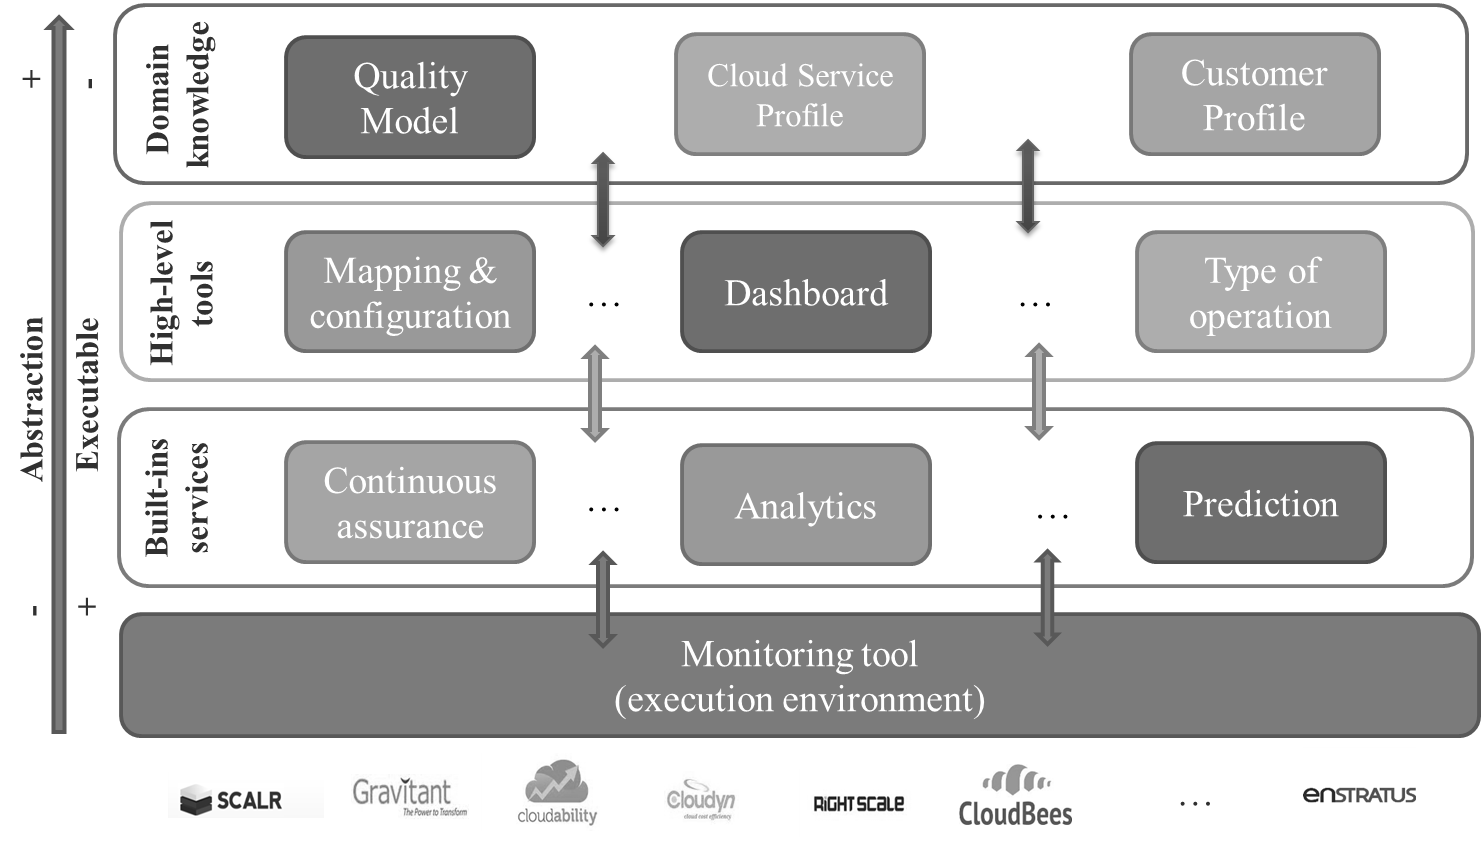
\includegraphics[width=12cm]{./imgs/qos-framework}
 \caption{QoS Framework.}
 \label{fig:qos-framework}
\end{figure}

On the other hand Figure~\ref{fig:lambda-qos} outlines the layers of the Lambda architecture (in this case the monitoring tool) with 
an adaptation to support semantics. 

\begin{itemize}
 \item \textbf{Batch layer.} It contains immutable, constantly growing dataset stored on a distributed file system like HDFS. This layer 
 receives as input the raw data coming from a queue. Data is then computed by means of some function and results are finally exposed 
 as batch views. As an extra step and with the aim of supporting the use of semantics these final views are promoted as RDF and thus SPARQL queries 
 can be executed on the computed results. This approach of adding an extra layer to ease queries over batch views has been 
 already address using SQL as a formal query language, e.g. SploutSQL. In this case SPARQL and RDF is selected to support the implicit 
 creation of queries from a semantic model. This layer is usually implemented using a MapReduce-based framework such as Apache Hadoop or 
 a more high-level framework such as Apache Pig. A final remark in this layer lies in the off-line execution of the algorithms or functions 
 that eases the pre-computation of results when large dataset processing is required.
 
 \item \textbf{Serving layer.} The responsibility of this layer is to manage both batch and real-time views 
 with the aim of providing a way of querying and merging both views and populate results to be consumed by 
 a third-service. In this case, this layer is in charge of executing the SPARQL queries (using a federated extension~\cite{DBLP:journals/corr/RakhmawatiUKHH13} 
 such as SPARQL-FedX~\cite{DBLP:conf/esws/SchwarteHHSS11}) and publish the results as RDF. At a first glance this job does not require 
 random writers but must support batch updates and random reads. In this case the implementation of joining 
 results is also designed as a Storm/Trident topology to enable and distributed real-time updates.
%  However it can be extraordinarily simple (candidates could be ElephantDB or Voldemort).

\item \textbf{Speed layer.} It deals with new data to compensate or decrease the latency of the batch layer. 
Functions are deployed on some stream processing system such as Storm, S4 or Spark and results are finally 
exposed as RDF. The functionality provided by this layer is mainly the same as the batch-layer but removing 
the latency and affording a real-time query system. Once data is also processed and available in the batch 
view a synchronization process must remove data from the real-time views. In this case Apache Zookepper 
can be used to keep synchronization in a distributed system.
\end{itemize}

The ``semantized'' Lambda Architecture using RDF and SPARQL on top of the batch and real-time views enables 
the possibility of handling the complexity of Big Data systems by defining a clear set of principles. Specifically 
the use of semantics serve to integrate data under a common data model that can be queried using a formal 
query language such as SPARQL. Furthermore immutability, human fault-tolerance and re-computation basic principles 
that can be easily adopted with the Hadoop platform. Finally and depending on the real-time requirements of 
the system some parts can be omitted and integrated in a further stage.

\begin{figure}[!ht]
\centering
	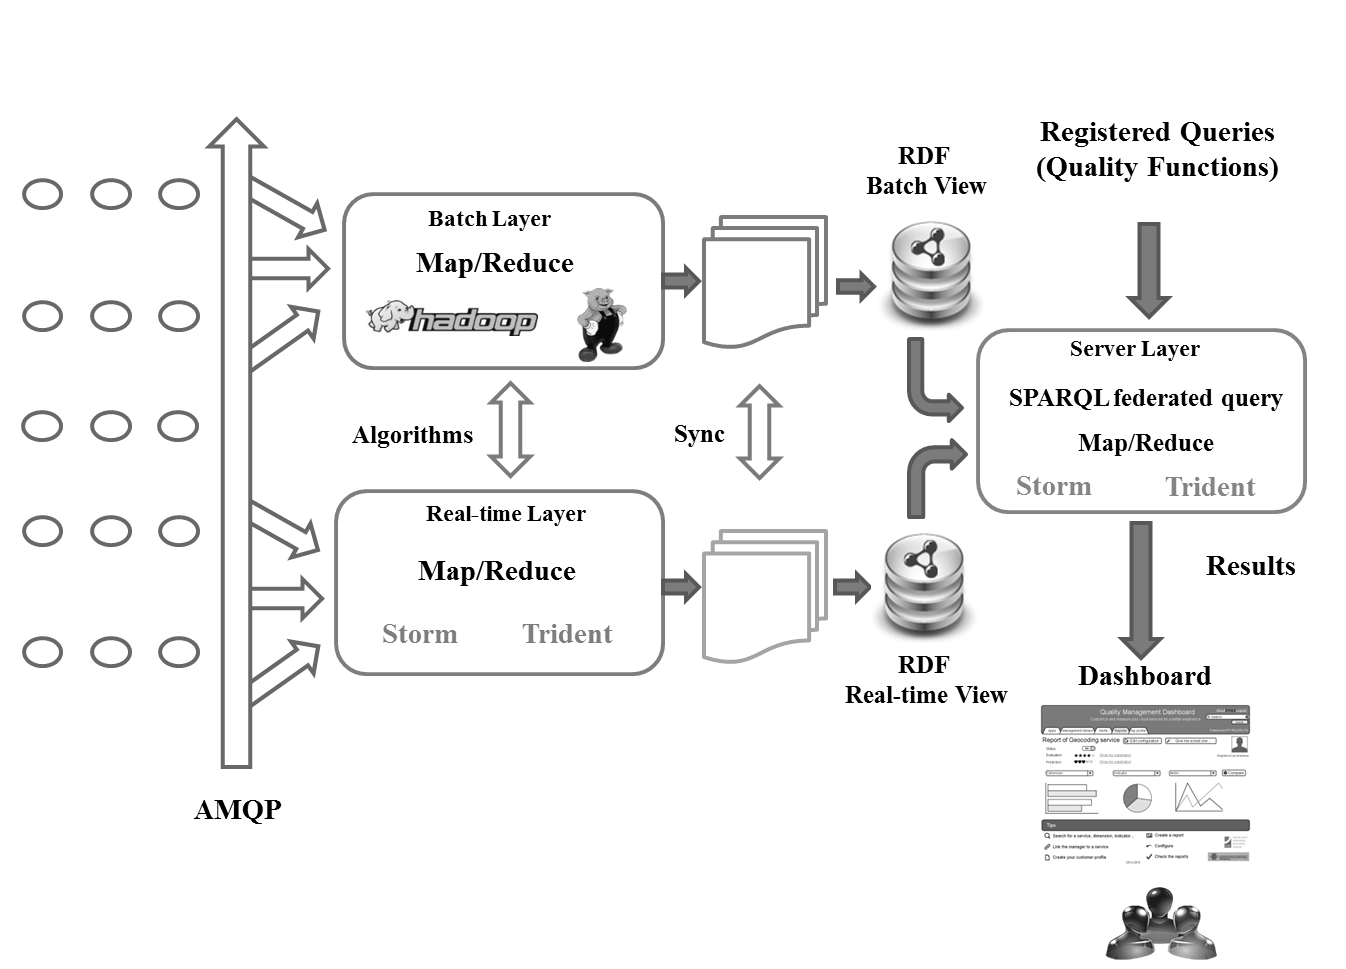
\includegraphics[width=12cm]{./imgs/lambda-qos}
 \caption{A semantic-based Lambda Architecture for real-time processing of diverse datastreams.}
 \label{fig:lambda-qos}
\end{figure}







% \section{Evaluation}\label{evaluation}
% \input{sections/evaluation}
\section{Discussion and Future Challenges}\label{discussion}
Despite the growing interest in Cloud Computing [102, 103] and the hype of this 
new paradigm for the creation of new era of applications, services and data 
available through the Web, a real advanced cloud management environment is far 
from being fully developed. There are many open issues to be solved and 
technology to ease the transition from traditional developments and applications 
to a cloud-based environment is still under development. With regards to QoS, 
there are a lot of initiatives and efforts trying to model and manage functional 
and non-functional properties in an intelligent fashion. Nevertheless the lack 
of standards for unifying information and data is preventing the deployment of 
advanced techniques for QoS management. In the case of semantic technologies, 
works in different areas are emerging to solve interoperability and integration 
problems in distributed environments. More specifically, the creation of 
knowledge-based systems applying semantic-based techniques as stream reasoning 
and CEP are currently being developed to deal mainly with Big Data problems in the 
context of social media or e-Government. Following a list of particular comments 
to discuss are presented:
\begin{itemize}
 \item There are a big variety of QoS dimensions to ensure in a cloud system. 
The methods to ensure reliability, security and trust should be modeled and 
discovered in automatic ways. In this specific case it is also required to take 
into account user feedback to evaluate the real quality and trust of a service. 
Moreover, depending on the cloud layer, specific QoS characteristics should be 
defined to collect the requirements of each particular case. Currently QoS 
approaches are mainly focused on web service discovery and selection but new 
ranking methods and reactive control systems taking into QoS features should be 
deployed to provide an intelligent cloud infrastructure.  

 \item Information about a service consists in both static and dynamic data, the 
matchmaking of services according to these issues is a key-enabler for a real 
QoS management but it is not fully addressed by existing works.

 \item According to Table  the big variety of ontologies, OWL models, etc. that 
have been designed in recent years imply a tangled set of options that should be 
unified to provide an unique view of  what QoS should be. Apart from that the 
use of semantics is not clear, in some cases reasoning processes are used to 
discover services but others just define an ontology as a proposal to provide a 
formal model without any real application. A clear semantic-based architecture 
[104, 105] should be defined containing the adequate definitions [106].of 
functional and non-functional properties.

 \item With regards to Semantic Web and reasoning, there is a growing community 
trying to provide technology for supporting intelligent systems in the new Web 
of Data. As a consequence the necessity of dealing with Big Data problems and 
data coming from different sources is stimulating the creation of new approaches 
to reuse existing technology such as Apache Hadoop in the context of querying 
large datasets. Therefore the main application of the Semantic Web principles 
lies in the unification of data and the execution of reasoning processes to 
validate data and infer new facts. Nevertheless, the existing logic formalisms 
available in OWL such as DL, FOL, F-Logic, etc. do not seem to be a solution to 
tackle the challenge of modeling dynamic domains that is why some works [107] 
regarding Continuous Semantics are emerging.

 \item A research area that is expected to play a key-role to enrich information 
is Linked Data. Currently this initiative has been successfully applied to 
information retrieval systems or in the creation of rich user interfaces. 
Nevertheless, the expectations of linking different datasets to enrich 
information are growing as a manner for delivering more intelligent services. To 
apply Linked Data in the Cloud Computing environment we should ensure that any 
resource to be monitored has an URI, its data is coded into RDF according to a 
formal model, an API or endpoint is accessible for fetching data using pulling 
pushing or triggering techniques and the methods for graph processing and 
reasoning are efficient and scalable under real-time constraints.
 
\end{itemize}

As main future challenge among others [108, 109], Semantics can help to increase 
the reliability in Cloud Computing providing the building blocks and models for 
an advanced QoS management. In the same way, Cloud Computing can help semantic 
technologies to be more scalable and flexible making use of the web as 
infrastructure to create large-scale data-intensive batch applications [110].


\section{Conclusions and Future work}\label{sect:conclusions}
An important body of work has been done during the last five years regarding the
deployment of cloud infrastructures, services and applications. As a result,
numerous SaaS, PaaS and IaaS providers can found as well as cloud management
platforms to ease the management of these infrastructures. In the same way, the
definition of QoS features in SOA has become a major research topic with a lot
of derived works trying to model and manage applying different approaches as
ontologies, rule based systems, etc. The arrival of new techniques for
processing real-time large and diverse datastreams from different data sources
to deliver ontology-based expert systems is very promising and the Cloud
Computing and the QoS management areas must take advantage of these methods to exploit cloud
infrastructures saving costs, being efficient and greener. Further steps require
the definition of a QoS model for cloud infrastructures and the design of
scalable infrastructures for connecting and managing resources on the cloud. The
market and business opportunities of this new realm are encouraging the research and the
collaboration between the academic and industrial areas fostering both the open
issues and the generated know-how among all interested parties.

\section{Acknowledgements}\label{sect:ack}
The research leading to these results has received funding from the European Union’s Seventh Framework Programme (FP7-PEOPLE-2010-ITN) 
under grant agreement n°264840 and developed in the context of the workpackage 4 and more specifically under the project 
``Quality Management in Service-based Systems and Cloud Applications''.



% 
% \nocite{*}
%\bibliographystyle{elsarticle-num}
\bibliographystyle{plain}
% % %\bibliographystyle{acm}
\bibliography{cloud-references,linked-data,references}
 % \renewcommand{\bibname}{References}


\end{document}
